%=================================================================
%=================================================================
\section{M11 Operations and Boundary Conditions}
%=================================================================
%=================================================================

\normalsize
%=================================================================
%=================================================================
Note that the last priority for each Control Definition will always evaluate to true. This will occur when none of the previous conditions evaluate to true. This is known as the 'default' condition.

The timestep for the MIKE11/MIKE1D model is a Fixed Time Step set to 2 minutes.

\clearpage
%=============================================================================================
\subsection{Boundary Conditions}
%=============================================================================================

This section lists open canal boundary conditions where water is added or removed from the M3ENP (MIKE11) domain. Canals with closed ends are not listed. This does not include river boundaries. These are points at the end of canals, and do not contain any control structures.

\scriptsize
\begin{table}[!h]
\centering
\caption{Summary of MIKE11 Boundary Conditions affecting Mass Balance}
\label{tab:M11BCfiles}
\begin{tabular}{llll}
\hline
\textbf{Canal} & \textbf{Location} & \textbf{Type}   & \textbf{File}     \\
\hline
 CLR\_025\_US    & N boundary  & Inflow          & $Q=0$ \\
 L-28            & N boundary  & Inflow          & BC\_S344\_Q.dfs0 \\
 L-29            & W boundary  & Water Level     & BC\_TAMIBR66.dfs0 \\
culvert\_42      & S boundary  & Inflow          & $Q=0$ \\
culvert\_43      & S boundary  & Inflow          & $Q=0$ \\
culvert\_44      & S boundary  & Inflow          & $Q=0$ \\
culvert\_45      & S boundary  & Inflow          & $Q=0$ \\
culvert\_46      & S boundary  & Inflow          & $Q=0$ \\
culvert\_47      & S boundary  & Inflow          & $Q=0$ \\
culvert\_48      & S boundary  & Inflow          & $Q=0$ \\
culvert\_49      & S boundary  & Inflow          & $Q=0$ \\
culvert\_50      & S boundary  & Inflow          & $Q=0$ \\
culvert\_51      & S boundary  & Inflow          & $Q=0$ \\
culvert\_52      & S boundary  & Inflow          & $Q=0$ \\
culvert\_53      & S boundary  & Inflow          & $Q=0$ \\
culvert\_54      & S boundary  & Inflow          & $Q=0$ \\
culvert\_55      & S boundary  & Inflow          & $Q=0$ \\
culvert\_56      & S boundary  & Inflow          & $Q=0$ \\
\\
culvert\_58      & S boundary  & Inflow          & $Q=0$ \\
culvert\_59      & S boundary  & Inflow          & $Q=0$ \\
 L-67\_A        & N boundary  & Water Level     & BC\_S12D\_HW.dfs0 \\
 L-30           & N boundary  & Water Level     & BC\_S335\_HW.dfs0 \\
 LPG2           & N boundary  & Inflow          & $Q=0$ \\
 LPG2           & S boundary  & Inflow          & $Q=0$ \\
 TTeastBridge   & S boundary  & Inflow          & $Q=0$ \\
 C-4            & E boundary  & Water Level     & BC\_G119TW.dfs0 \\
 C-1W           & E boundary  & Water Level     & BC\_S148\_TW.dfs0 \\
 C-102          & E boundary  & Water Level     & BC\_S194TW-S165HW.dfs0 \\
 C-103N         & E boundary  & Water Level     & BC\_S166\_HW.dfs0 \\
 C-103          & E boundary  & Water Level     & BC\_S179\_HW.dfs0 \\
 C-111          & S boundary  & Water Level     & BC\_S197\_TW.dfs0 \\
\hline
\end{tabular}
\end{table}
\normalsize


\clearpage
%=============================================================================================
\subsection{Operations: L-67A, L-67C, and Pocket Canals}
%=============================================================================================

%----------------------------------------------------------
\subsubsection{L-67A}
%----------------------------------------------------------

In the model, the northern boundary of L67A is a head boundary, with prescribed timeseries of S12D\_HW.

The Pocket canal intersects with L67A near the center of the canal.

The southern boundary of L67A is connected to L29 between S333 and S12D.

%\begin{figure}[!ht] \begin{center}
%  \includegraphics[width=6.5in]{../figs/timeseries/S12D_HW.png}
%  \caption{Prescribed Flow at L67A North Boundary}\label{fig:S12D_HW:STRUCTURE}\end{center}
%\end{figure}

\clearpage

%----------------------------------------------------------
\subsubsection{L-67C}
%----------------------------------------------------------
The north boundary of L67C is closed.

The Pocket canal intersects with L67C near the center of the canal.

The southern end of L67C is connected with L67A.

\clearpage

%----------------------------------------------------------
\subsubsection{The Pocket}
%----------------------------------------------------------

The pocket canal has no control structures or boundary conditions, and has open connections with L67A and L67C at both ends.
%The east boundary of this canal is closed, and the west boundary of the canal is a prescribed head timeseries, shown in Figure~\ref{fig:tsr79c49_HW:STRUCTURE}. It is derived from the timeseries output for Row 79 and Column 49, we think.

%\begin{figure}[!ht] \begin{center}
%  \includegraphics[width=6.5in]{../figs/timeseries/tsr79c49.png}
%  \caption{Prescribed Flow at West Boundary of the Pocket Canal}\label{fig:tsr79c49_HW:STRUCTURE}\end{center}
%\end{figure}

\clearpage

%=============================================================================================
\subsection{Operations: Tram Road Canals (ROAD\_SRS and ROAD\_SRS\_E}
%=============================================================================================
\begin{figure}[!h]
  \begin{center}
  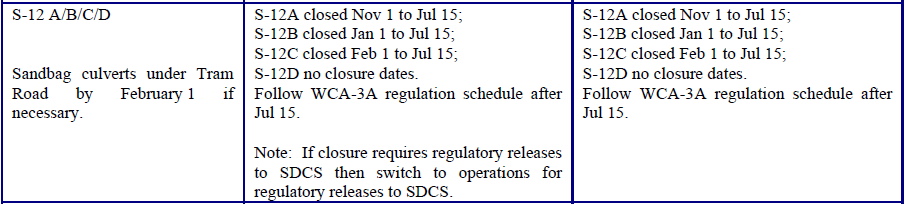
\includegraphics[width=6.5in]{../figs/S12s_IOPops.png}
  \caption{Tram Road Culverts IOP Operations}
  \label{fig:TRCiop}
  \end{center}
\end{figure}

Currently there are no culverts in this road in the model, therefore no operations.

The model also does not include the four barrel culverts in the Old Tamiami Trail Borrow canal under the north end of the Tram Road, or the structure connecting the Tram road borrow canal to the Old Tamiami Trail borrow canal.

\clearpage
%=============================================================================================
\subsection{Operations: L-29 Canal}
%=============================================================================================

%----------------------------------------------------------
\subsubsection{S343A}
%----------------------------------------------------------

This structure is implemented in MIKE 1D as a Discharge structure with a Max Rate of change of 1 $cfs/s$.

\begin{figure}[!h]
  \begin{center}
  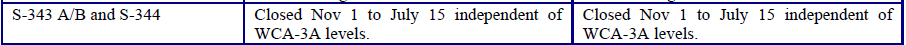
\includegraphics[width=6.5in]{../figs/S343-S344_IOPops.png}
  \caption{Tram Road Culverts IOP Operations}
  \label{fig:343iop}
  \end{center}
\end{figure}

The M11 model implements this structure with prescribed flow.

\begin{packed_items}
\item Priority 1: $Q = Q_{obs}$
\end{packed_items}

%\begin{figure}[!ht] \begin{center}
%  % Requires \usepackage{graphicx}
%  \includegraphics[width=6.5in]{MODEL/FIGURE/S343A_HW_TS.png}
%  \caption[Headwater at structure S343A]{Headwater at structure S343A}\label{fig:S343A_HW:STRUCTURE}\end{center}
%\end{figure}
%
%\begin{figure}[!ht] \begin{center}
%  % Requires \usepackage{graphicx}
%  \includegraphics[width=6.5in]{MODEL/FIGURE/S343A_HW_TS.png}
%  \caption[Tailwater at structure S343A]{Tailwater at structure S343A}\label{fig:S343A_TW:STRUCTURE}\end{center}
%\end{figure}
%
%\begin{figure}[!ht] \begin{center}
%  % Requires \usepackage{graphicx}
%  \includegraphics[width=6.5in]{MODEL/FIGURE/S343A_Q_TS.png}
%  \caption[Flowrate at structure S343A]{Flowrate at structure S343A}\label{fig:S343A_Q:STRUCTURE}\end{center}
%\end{figure}
%
%\begin{figure}[!ht] \begin{center}
%  % Requires \usepackage{graphicx}
%  \includegraphics[width=6.5in]{MODEL/FIGURE/S343A_Q-acc.png}
%  \caption[Cumulative flow at structure S343A]{Cumulative flow at structure S343A}\label{fig:S343A_QACC:STRUCTURE}\end{center}
%\end{figure}

\clearpage

%----------------------------------------------------------
\subsubsection{S343B}
%----------------------------------------------------------

This structure is implemented in MIKE 1D as a Discharge structure with a Max Rate of change of 1 $cfs/s$.

\begin{figure}[!h]
  \begin{center}
  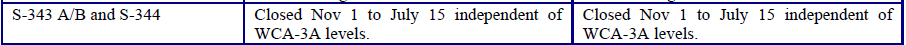
\includegraphics[width=6.5in]{../figs/S343-S344_IOPops.png}
  \caption{Tram Road Culverts IOP Operations}
  \label{fig:343iop}
  \end{center}
\end{figure}

The M11 model implements this structure with prescribed flow.

\begin{packed_items}
\item Priority 1: $Q = Q_{obs}$
\end{packed_items}

%\begin{figure}[!ht] \begin{center}
%  % Requires \usepackage{graphicx}
%  \includegraphics[width=6.5in]{MODEL/FIGURE/S343B_HW_TS.png}
%  \caption[Headwater at structure S343B]{Headwater at structure S343B}\label{fig:S343B_HW:STRUCTURE}\end{center}
%\end{figure}
%
%\begin{figure}[!ht] \begin{center}
%  % Requires \usepackage{graphicx}
%  \includegraphics[width=6.5in]{MODEL/FIGURE/S343B_HW_TS.png}
%  \caption[Tailwater at structure S343B]{Tailwater at structure S343B}\label{fig:S343B_TW:STRUCTURE}\end{center}
%\end{figure}
%
%\begin{figure}[!ht] \begin{center}
%  % Requires \usepackage{graphicx}
%  \includegraphics[width=6.5in]{MODEL/FIGURE/S343B_Q_TS.png}
%  \caption[Flowrate at structure S343B]{Flowrate at structure S343B}\label{fig:S343B_Q:STRUCTURE}\end{center}
%\end{figure}
%
%\begin{figure}[!ht] \begin{center}
%  % Requires \usepackage{graphicx}
%  \includegraphics[width=6.5in]{MODEL/FIGURE/S343B_Q-acc.png}
%  \caption[Cumulative flow at structure S343B]{Cumulative flow at structure S343B}\label{fig:S343B_QACC:STRUCTURE}\end{center}
%\end{figure}

\clearpage

%----------------------------------------------------------
\subsubsection{L-29 western boundary}
%----------------------------------------------------------


\clearpage
%----------------------------------------------------------
\subsubsection{Culverts 24-28}

The M11 model implements each of these culverts with prescribed flow.

\begin{packed_items}
\item Priority 1: $Q = Q_{obs}$
\end{packed_items}

%----------------------------------------------------------

%Flow timeseries for culverts shown in Figures~\ref{fig:culv24Q:STRUCTURE}-\ref{fig:culv28Q:STRUCTURE}.
%
%\begin{figure}[!ht] \begin{center}
%  \includegraphics[width=6.5in]{../figs/timeseries/CULVERT-24_Q.png}
%  \caption{Prescribed Flow at Culvert 24}\label{fig:culv24Q:STRUCTURE}\end{center}
%\end{figure}
%
%\begin{figure}[!ht] \begin{center}
%  \includegraphics[width=6.5in]{../figs/timeseries/CULVERT-25_Q.png}
%  \caption{Prescribed Flow at Culvert 25}\label{fig:culv25Q:STRUCTURE}\end{center}
%\end{figure}
%
%\begin{figure}[!ht] \begin{center}
%  \includegraphics[width=6.5in]{../figs/timeseries/CULVERT-26_Q.png}
%  \caption{Prescribed Flow at Culvert 26}\label{fig:culv26Q:STRUCTURE}\end{center}
%\end{figure}
%
%\begin{figure}[!ht] \begin{center}
%  \includegraphics[width=6.5in]{../figs/timeseries/CULVERT-27_Q.png}
%  \caption{Prescribed Flow at Culvert 27}\label{fig:culv27Q:STRUCTURE}\end{center}
%\end{figure}
%
%\begin{figure}[!ht] \begin{center}
%  \includegraphics[width=6.5in]{../figs/timeseries/CULVERT-28_Q.png}
%  \caption{Prescribed Flow at Culvert 28}\label{fig:culv28Q:STRUCTURE}\end{center}
%\end{figure}


\clearpage
%----------------------------------------------------------
\subsubsection{S14}
%----------------------------------------------------------
Not in model.

\clearpage
%----------------------------------------------------------
\subsubsection{S12A-D}
%----------------------------------------------------------

These four structures are reinforced concrete, gated spillways with the discharge of each controlled by six cable operated, vertical lift gates. Operation of gates is manually controlled, and the gates are operated in accordance with the seasonal operational criteria. The structures are located in Levee 29 (U.S. Highway 41) on the south perimeter of Conservation Area 3A, about 30 miles west of Miami. These structures provide the principal means of discharge from Conservation Area 3A. Relatively minor discharge can also be made by S-151 into Conservation Area 3B. Structures 12A, B, C, and D provide the principal means of discharge to the Everglades National Park.

%\paragraph{IOP Operational Guidance}
%
%Column 1:
%\begin{packed_items}
%\item S-12A closed Nov 1 to Jul 15;
%\item S-12B closed Jan 1 to Jul 15;
%\item S-12C closed Feb 1 to Jul 15;
%\item S-12D no closure dates.
%\item Follow WCA-3A regulation schedule after Jul 15.
%\item Note: If closure requires regulatory releases to SDCS then switch to operations for regulatory releases to SDCS.
%\end{packed_items}
%
%Column 2:
%\begin{packed_items}
%\item S-12A closed Nov 1 to Jul 15;
%\item S-12B closed Jan 1 to Jul 15;
%\item S-12C closed Feb 1 to Jul 15;
%\item S-12D no closure dates.
%\item Follow WCA-3A regulation schedule after Jul 15.
%\end{packed_items}

\begin{figure}[!h]
  \begin{center}
  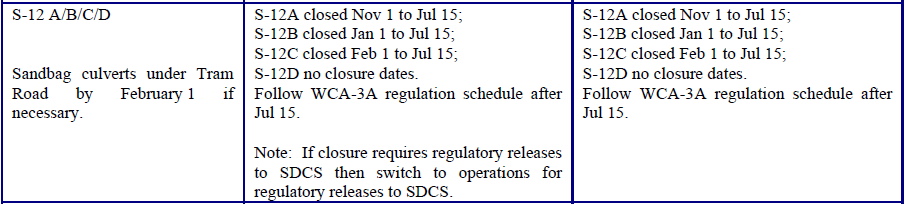
\includegraphics[width=6.5in]{../figs/S12s_IOPops.png}
  \caption{Tram Road Culverts IOP Operations}
  \label{fig:S12siop}
  \end{center}
\end{figure}

\begin{packed_items}
\item Priority 1: $Q = Q_{obs}$
\end{packed_items}


%\begin{figure}[!ht] \begin{center}
%  % Requires \usepackage{graphicx}
%  \includegraphics[width=6.5in]{MODEL/FIGURE/S12A_HW_TS.png}
%  \caption[Headwater at structure S12A]{Headwater at structure S12A}\label{fig:S12A_HW:STRUCTURE}\end{center}
%\end{figure}
%
%\begin{figure}[!ht] \begin{center}
%  % Requires \usepackage{graphicx}
%  \includegraphics[width=6.5in]{MODEL/FIGURE/S12A_TW_TS.png}
%  \caption[Tailwater at structure S12A]{Tailwater at structure S12A}\label{fig:S12A_TW:STRUCTURE}\end{center}
%\end{figure}
%
%\begin{figure}[!ht] \begin{center}
%  % Requires \usepackage{graphicx}
%  \includegraphics[width=6.5in]{MODEL/FIGURE/S12A_Q_TS.png}
%  \caption[Flowrate at structure S12A]{Flowrate at structure S12B}\label{fig:S12B_Q:STRUCTURE}\end{center}
%\end{figure}

%\begin{figure}[!ht] \begin{center}
%  % Requires \usepackage{graphicx}
%  \includegraphics[width=6.5in]{MODEL/FIGURE/S12A_Q-acc.png}
%  \caption[Accumulated flow at structure S12A]{Accumulated flow at structure S12B}\label{fig:S12A_Q:ACC}\end{center}
%\end{figure}

%\begin{figure}[!ht] \begin{center}
%  % Requires \usepackage{graphicx}
%  \includegraphics[width=6.5in]{MODEL/FIGURE/S12B_HW_TS.png}
%  \caption[Headwater at structure S12B]{Headwater at structure S12B}\label{fig:S12B_HW:STRUCTURE}\end{center}
%\end{figure}
%
%\begin{figure}[!ht] \begin{center}
%  % Requires \usepackage{graphicx}
%  \includegraphics[width=6.5in]{MODEL/FIGURE/S12B_TW_TS.png}
%  \caption[Tailwater at structure S12B]{Tailwater at structure S12B}\label{fig:S12B_TW:STRUCTURE}\end{center}
%\end{figure}
%
%\begin{figure}[!ht] \begin{center}
%  % Requires \usepackage{graphicx}
%  \includegraphics[width=6.5in]{MODEL/FIGURE/S12B_Q_TS.png}
%  \caption[Flowrate at structure S12B]{Flowrate at structure S12B}\label{fig:S12B_Q:STRUCTURE}\end{center}
%\end{figure}

%\begin{figure}[!ht] \begin{center}
%  % Requires \usepackage{graphicx}
%  \includegraphics[width=6.5in]{MODEL/FIGURE/S12B_Q-acc.png}
%  \caption[Accumulated flow at structure S12B]{Accumulated flow at structure S12B}\label{fig:S12B_Q:ACC}\end{center}
%\end{figure}

%\begin{figure}[!ht] \begin{center}
%  % Requires \usepackage{graphicx}
%  \includegraphics[width=6.5in]{MODEL/FIGURE/S12C_HW_TS.png}
%  \caption[Headwater at structure S12C]{Headwater at structure S12A}\label{fig:S12C_HW:STRUCTURE}\end{center}
%\end{figure}
%
%\begin{figure}[!ht] \begin{center}
%  % Requires \usepackage{graphicx}
%  \includegraphics[width=6.5in]{MODEL/FIGURE/S12C_TW_TS.png}
%  \caption[Tailwater at structure S12C]{Tailwater at structure S12A}\label{fig:S12C_TW:STRUCTURE}\end{center}
%\end{figure}
%
%\begin{figure}[!ht] \begin{center}
%  % Requires \usepackage{graphicx}
%  \includegraphics[width=6.5in]{MODEL/FIGURE/S12C_Q_TS.png}
%  \caption[Flowrate at structure S12C]{Flowrate at structure S12A}\label{fig:S12C_Q:STRUCTURE}\end{center}
%\end{figure}

%\begin{figure}[!ht] \begin{center}
%  % Requires \usepackage{graphicx}
%  \includegraphics[width=6.5in]{MODEL/FIGURE/S12C_Q-acc.png}
%  \caption[Accumulated flow at structure S12C]{Accumulated flow at structure S12C}\label{fig:S12C_Q:ACC}\end{center}
%\end{figure}

%\begin{figure}[!ht] \begin{center}
%  % Requires \usepackage{graphicx}
%  \includegraphics[width=6.5in]{MODEL/FIGURE/S12D_HW_TS.png}
%  \caption[Headwater at structure S12D]{Headwater at structure S12D}\label{fig:S12D_HW:STRUCTURE}\end{center}
%\end{figure}
%
%\begin{figure}[!ht] \begin{center}
%  % Requires \usepackage{graphicx}
%  \includegraphics[width=6.5in]{MODEL/FIGURE/S12D_TW_TS.png}
%  \caption[Tailwater at structure S12D]{Tailwater at structure S12D}\label{fig:S12D_TW:STRUCTURE}\end{center}
%\end{figure}
%
%\begin{figure}[!ht] \begin{center}
%  % Requires \usepackage{graphicx}
%  \includegraphics[width=6.5in]{MODEL/FIGURE/S12D_Q_TS.png}
%  \caption[Flowrate at structure S12D]{Flowrate at structure S12D}\label{fig:S12D_Q:STRUCTURE}\end{center}
%\end{figure}

%\begin{figure}[!ht] \begin{center}
%  % Requires \usepackage{graphicx}
%  \includegraphics[width=6.5in]{MODEL/FIGURE/S12D_Q-acc.png}
%  \caption[Accumulated flow at structure S12D]{Accumulated flow at structure S12D}\label{fig:S12D_Q:ACC}\end{center}
%\end{figure}

\clearpage
%----------------------------------------------------------
\subsubsection{S333}
%----------------------------------------------------------

\paragraph{SFWMD Structure Book Description, rev. 1/10/2000}
S333 is operated to make releases from Conservation Area 3A into the Tamiami Canal.

Purpose:
This structure functions principally to make water deliveries from Conservation Area 3A to south and eastern Dade County to Shark River and Taylor Slough areas of the Everglades National Park. It can be used to make regulation releases from Conservation Area 3A. This structure is implemented in MIKE 1D as an Underflow structure.

%%Operating Criteria:
%%When this structure is operated to make deliveries to south or east Dade County from Conservation Area 3, it may be operated alone or with S-337. The total delivery will be the amount necessary to maintain the appropriate stages at S-331, S-25B and S-22. During such transfer operations, the headwater stage at S-334 will be maintained between 5.0 and 6.0.
%%
%%When S-333 is used in conjunction with S-12 to make regulatory releases to the Everglades National Park at Shark River Slough, the structure will be operated in accordance with Iteration 7, Experimental Program of Water Deliveries to Everglades National Park, dated the 5th day of October, 1995, between the Corps of Engineers, the Everglades National Park, and the District. Iteration 7 commenced on November 1, 1995.
%%    (1) S-333 discharges would be limited to avoid causing the downstream water levels to exceed 7.5 ft., NGVD.
%%    (2) When water levels at G-3273 have been above 6.8 feet, NGVD for 24 hours, S-333 will be closed.
%%    (3) S-333 will be closed until the water level at G-3273 has stopped rising and is below 6.8 ft., NGVD if the following conditions occur:
%%        (a) The water level at G-3273 has been above 6.5 ft., NGVD for 48 hours; and
%%        (b) The water level at G-3273 has risen in the last 24 hours at a rate that would cause it to exceed 6.8 ft., NGVD, within the next 24 hours.
%%    (4) If the headwater stage at S-176 exceeds 5.0 ft., NGVD for more than 24 hours or the S-331 headwater stage exceeds its target level for more than 24 hours, discharges at S-333 will be reduced, if necessary, to avoid causing water levels in the L-29 borrow canal from exceeding 7.25 ft., NGVD until stages at S-331 and S-176 have been maintained at the appropriate levels for 24 hours.
%%
%%Discharges to Shark River Slough of the Everglades National Park are a function of a rain
%%driven model. The quantities are determined weekly by the Corps of Engineers and given by telecom
%%each Monday, to be implemented by the District on Tuesday.
%%
%%Weir Crest: Net Length 29 feet, Elevation -3.1 feet
%%Service Bridge Elevation 14.5 feet
%%Water Level which will by-pass structure 14.5 feet
%%Gates:
%%    Number 1
%%    Size 14.6 ft. high by 29 ft. wide
%%    Type vertical lift gate
%%    Bottom elevation of gates, full open 8.5 feet

\begin{figure}[!h]
  \begin{center}
  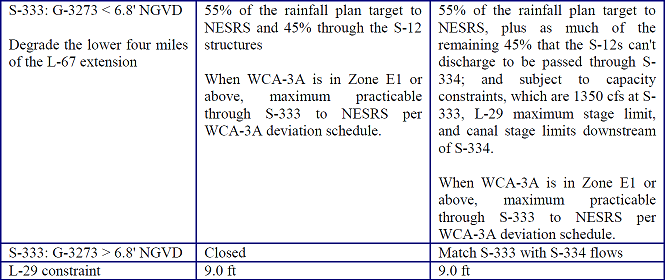
\includegraphics[width=6.5in]{../figs/S333_IOPops.png}
  \caption{S333 IOP Operations}
  \label{fig:S333iop}
  \end{center}
\end{figure}

%Column 1 (G-3273 $<$ 6.8' NGVD):
%\begin{packed_items}
%\item 55\% of the rainfall plan target to NESRS and 45\% through the S-12 structures
%\item When WCA-3A is in Zone E1 or above, maximum practicable through S-333 to NESRS per WCA-3A deviation schedule.
%\end{packed_items}
%
%
%Column 2 (G-3273 $<$ 6.8' NGVD):
%\begin{packed_items}
%\item 55\% of the rainfall plan target to NESRS, plus as much of the remaining 45\% that the S-12s can't discharge to be passed through S-334 and subject to capacity constraints, which are 1350 cfs at S-333, L-29 maximum stage limit, and canal stage limits downstream of S-334.
%\item When WCA-3A is in Zone E1 or above, maximum practicable through S-333 to NESRS per WCA-3A deviation schedule.
%\end{packed_items}
%
%Column 1 (G-3273 $>$ 6.8' NGVD): Closed.
%
%Column 2 (G-3273 $>$ 6.8' NGVD): Match S-333 with S-334 flows.



The M11 model implements this structure using a prescribed tailwater timeseries, i.e. the structure passes the required amount of water to maintain the tailwater at the structure equal to observed timeseries. For modeling operations at S333 it will be necessary to implement operations that are controlled by stages in WCA3A.

%\begin{figure}[!ht] \begin{center}
%  \includegraphics[width=6.5in]{../figs/timeseries/S333_TW.png}
%  \caption{Prescribed Tailwater at Structure S333}
%  \label{fig:S333TW:STRUCTURE}\end{center}
%\end{figure}

The Max speed for gate opening is 0.000138 ft/sec, which equals 0.01656 ft per 2-minute timestep.

\begin{packed_items}
\item Priority 1: If $Mode=1$ and $H_{ds}<S333\_TW_{obs}$,  and $Q_{str}<1300$ cfs,  operate according to Table~\ref{tab:CS-S333open}.
\item Priority 2: If $Mode=1$ and $H_{ds}>S333\_TW_{obs}$,  operate according to Table~\ref{tab:CS-S333close}.
\item[]
\item Priority 3: If $Mode=2$ and $H_{ds}<S333\_TW_{obs}$,  and $Q_{str}<1300$ cfs,,  operate according to Table~\ref{tab:CS-S333open}.
\item Priority 4: If $Mode=2$ and $H_{ds}>S333\_TW_{obs}$,  operate according to Table~\ref{tab:CS-S333close}.
\item[]
\item Priority 5: If $Mode=0$ and $H_{ds}<S333\_TW_{obs}$, and $Q_{str}<1300$ cfs,  operate according to Table~\ref{tab:CS-S333open}.
\item Priority 6: If $Mode=0$ and $H_{ds}>S333\_TW_{obs}$,  operate according to Table~\ref{tab:CS-S333close}.
\item[]
\item Priority 7: If $H<0$, operate according to Table~\ref{tab:CS-S333close}.
\end{packed_items}

\footnotesize
\begin{table}[!h]
\centering
\caption{Control strategy for S333 open (units are ft. NGVD29)}
\label{tab:CS-S333open}
\begin{tabular}{p{1.2in}{r} p{0.5in}{r}}
\hline
\textbf{Current Gate Level} & \textbf{Gate Level}\\
\hline
-3.1	& -3       \\
8.4	& 8.5   \\
\hline
\end{tabular}
\end{table}
\normalsize

\footnotesize
\begin{table}[!h]
\centering
\caption{Control strategy for S333 close (Units are ft. NGVD29)}
\label{tab:CS-S333close}
\begin{tabular}{p{1.2in}{r} p{0.5in}{r}}
\hline
\textbf{Current Gate Level} & \textbf{Gate Level}\\
\hline
-3	& -3.1       \\
8.5	& 8.4   \\
\hline
\end{tabular}
\end{table}
\normalsize


%\begin{figure}[!ht] \begin{center}
%  % Requires \usepackage{graphicx}
%  \includegraphics[width=6.5in]{MODEL/FIGURE/S333_HW_TS.png}
%  \caption[Headwater at structure S333]{Headwater at structure S333}\label{fig:S333_HW:STRUCTURE}\end{center}
%\end{figure}
%
%\begin{figure}[!ht] \begin{center}
%  % Requires \usepackage{graphicx}
%  \includegraphics[width=6.5in]{MODEL/FIGURE/S333_HW_TS.png}
%  \caption[Tailwater at structure S333]{Tailwater at structure S333}\label{fig:S333_TW:STRUCTURE}\end{center}
%\end{figure}
%
%\begin{figure}[!ht] \begin{center}
%  % Requires \usepackage{graphicx}
%  \includegraphics[width=6.5in]{MODEL/FIGURE/S333_Q_TS.png}
%  \caption[Flowrate at structure S333]{Flowrate at structure S333}\label{fig:S333_Q:STRUCTURE}\end{center}
%\end{figure}

%\begin{figure}[!ht] \begin{center}
%  % Requires \usepackage{graphicx}
%  \includegraphics[width=6.5in]{MODEL/FIGURE/S333_Q-acc.png}
%  \caption[Cumulative flow at structure S333]{Cumulative flow at structure S333}\label{fig:S333_QACC:STRUCTURE}\end{center}
%\end{figure}

\clearpage
%----------------------------------------------------------
\subsubsection{Culverts 41-59}
%----------------------------------------------------------

Culverts 41-59 are implemented in the model as both Culvert structures and Control Structures. Each is described below. The Tamiami Trail Bridge is one mile long, and replaced Culvert 57 when it was built. (Note: Section Type for all culverts is 'closed', meaning the roof of the culvert is not open to the air above.)

\paragraph{Culverts:}

\begin{itemize}

\item Culverts \textcolor[rgb]{1.00,0.00,0.00}{52, 56}, 57, and \textcolor[rgb]{1.00,0.00,0.00}{58}: Valve Regulation is 'closed', meaning no flow is allowed through this culvert.

\item All other Culverts: Valve Regulation is 'none', meaning flow is allowed in both directions.


\end{itemize}

\paragraph{Control Structures:}

\begin{itemize}

\item Culverts 41-56 and 58-59:

\begin{packed_items}
\item Priority 1: Closed
\end{packed_items}

\item Culvert 57 is not in the model as a Control Structure.

\end{itemize}

%Historical note: There are potential occurrences when flow is backwards from NESS into L-29 canal through culverts 41 to 48 in the observed data.
%
%Culverts 41-59 are implemented as passive culverts allowing flow.
%Between 2010-2013, Culvert 57 was removed when the Tamiami Trail bridge was installed.
%
%Culverts 41-59 are all implemented as control structures with prescribed flow timeseries, see Figures~\ref{fig:culv41Q:STRUCTURE}-~\ref{fig:culv59Q:STRUCTURE}. The data source for this data is unknown.
%
%\begin{figure}[!hp] \begin{center} \includegraphics[width=6.5in]{../figs/timeseries/CULVERT-41_Q.png} \caption{Prescribed Flow at Culvert 41}\label{fig:culv41Q:STRUCTURE}\end{center}\end{figure}
%\begin{figure}[!hp] \begin{center} \includegraphics[width=6.5in]{../figs/timeseries/CULVERT-42_Q.png} \caption{Prescribed Flow at Culvert 42}\label{fig:culv42Q:STRUCTURE}\end{center}\end{figure}
%\begin{figure}[!hp] \begin{center} \includegraphics[width=6.5in]{../figs/timeseries/CULVERT-43_Q.png} \caption{Prescribed Flow at Culvert 43}\label{fig:culv43Q:STRUCTURE}\end{center}\end{figure}
%\clearpage
%\begin{figure}[!hp] \begin{center} \includegraphics[width=6.5in]{../figs/timeseries/CULVERT-44_Q.png} \caption{Prescribed Flow at Culvert 44}\label{fig:culv44Q:STRUCTURE}\end{center}\end{figure}
%\begin{figure}[!hp] \begin{center} \includegraphics[width=6.5in]{../figs/timeseries/CULVERT-45_Q.png} \caption{Prescribed Flow at Culvert 45}\label{fig:culv45Q:STRUCTURE}\end{center}\end{figure}
%\begin{figure}[!hp] \begin{center} \includegraphics[width=6.5in]{../figs/timeseries/CULVERT-46_Q.png} \caption{Prescribed Flow at Culvert 46}\label{fig:culv46Q:STRUCTURE}\end{center}\end{figure}
%\clearpage
%\begin{figure}[!hp] \begin{center} \includegraphics[width=6.5in]{../figs/timeseries/CULVERT-47_Q.png} \caption{Prescribed Flow at Culvert 47}\label{fig:culv47Q:STRUCTURE}\end{center}\end{figure}
%\begin{figure}[!hp] \begin{center} \includegraphics[width=6.5in]{../figs/timeseries/CULVERT-48_Q.png} \caption{Prescribed Flow at Culvert 48}\label{fig:culv48Q:STRUCTURE}\end{center}\end{figure}
%\begin{figure}[!hp] \begin{center} \includegraphics[width=6.5in]{../figs/timeseries/CULVERT-49_Q.png} \caption{Prescribed Flow at Culvert 49}\label{fig:culv49Q:STRUCTURE}\end{center}\end{figure}
%\clearpage
%\begin{figure}[!hp] \begin{center} \includegraphics[width=6.5in]{../figs/timeseries/CULVERT-50_Q.png} \caption{Prescribed Flow at Culvert 50}\label{fig:culv50Q:STRUCTURE}\end{center}\end{figure}
%\begin{figure}[!hp] \begin{center} \includegraphics[width=6.5in]{../figs/timeseries/CULVERT-51_Q.png} \caption{Prescribed Flow at Culvert 51}\label{fig:culv51Q:STRUCTURE}\end{center}\end{figure}
%\begin{figure}[!hp] \begin{center} \includegraphics[width=6.5in]{../figs/timeseries/ReplaceMe.png} \caption{Prescribed Flow at Culvert 52}\label{fig:culv52Q:STRUCTURE}\end{center}\end{figure}
%\clearpage
%\begin{figure}[!hp] \begin{center} \includegraphics[width=6.5in]{../figs/timeseries/CULVERT-53_Q.png} \caption{Prescribed Flow at Culvert 53}\label{fig:culv53Q:STRUCTURE}\end{center}\end{figure}
%\begin{figure}[!hp] \begin{center} \includegraphics[width=6.5in]{../figs/timeseries/CULVERT-54_Q.png} \caption{Prescribed Flow at Culvert 54}\label{fig:culv54Q:STRUCTURE}\end{center}\end{figure}
%\begin{figure}[!hp] \begin{center} \includegraphics[width=6.5in]{../figs/timeseries/CULVERT-55_Q.png} \caption{Prescribed Flow at Culvert 55}\label{fig:culv55Q:STRUCTURE}\end{center}\end{figure}
%\clearpage
%\begin{figure}[!hp] \begin{center} \includegraphics[width=6.5in]{../figs/timeseries/ReplaceMe.png} \caption{Prescribed Flow at Culvert 56}\label{fig:culv56Q:STRUCTURE}\end{center}\end{figure}
%\begin{figure}[!hp] \begin{center} \includegraphics[width=6.5in]{../figs/timeseries/CULVERT-57_Q.png} \caption{Prescribed Flow at Culvert 57}\label{fig:culv57Q:STRUCTURE}\end{center}\end{figure}
%\begin{figure}[!hp] \begin{center} \includegraphics[width=6.5in]{../figs/timeseries/ReplaceMe.png} \caption{Prescribed Flow at Culvert 58}\label{fig:culv58Q:STRUCTURE}\end{center}\end{figure}
%\clearpage
%\begin{figure}[!hp] \begin{center} \includegraphics[width=6.5in]{../figs/timeseries/CULVERT-59_Q.png} \caption{Prescribed Flow at Culvert 59}\label{fig:culv59Q:STRUCTURE}\end{center}\end{figure}
%

\clearpage
%----------------------------------------------------------
\subsubsection{Tamiami Trail Bridge}
%----------------------------------------------------------
Name: TTeastBridge

Implemented in the model as a Weir.


\clearpage
%----------------------------------------------------------
\subsubsection{S334}
%----------------------------------------------------------
S-334 allows water to be delivered from L-29 to L-31N and is used for both water supply and flood control.
Since IOP and under ERTP the structure has been increasingly used to in an attempt to lower water levels of WCA-3A.
This "wrap-around" strategy delivers water into L-31N and is pumped into the detention areas in addition to the local flood control pumping.
The "column II operation" is designed to bypass ENP wetlands which may be too wet, i.e. water level is above ground surface in the principal historical slough area, Northeast Shark Slough (NESS).

\paragraph{SFWMD Structure Book Description, rev. 3/30/1999}
This structure functions principally to make supplemental water deliveries to South and East Dade County.
It can also be used when regulatory releases from Conservation Area 3A are being made.
This structure is operated in conjunction with S-335 to make supplemental deliveries to South and East Dade County.
S-335 is the primary structure to deliver water.
During such transfer operations, the headwater stage at S-334 is maintained between 5.0 and 6.0.
When supplemental deliveries are not being made, this structure is closed.
When regulatory releases are being made from Conservation Area 3A, this structure is operated in conjunction with S-333 to maintain a maximum stage of 7.05 ft at the L-29-1 culvert \cite{corp2005, SFWMD1994}.
Higher stages cause flooding at the Indian Village adjacent to the canal.

This structure is set to Underflow.

%Weir Crest
%    Net Length 29.0 feet
%    Elevation -6.9 feet
%Service bridge elevation 14.0
%Water level which will bypass structure 14.0 feet
%Gates
%    Number 1
%    Size 17 ft. high by 29.0 ft. wide

\begin{figure}[!h]
  \begin{center}
  \includegraphics[width=6.5in]{../figs/S334_IOPops.png}
  \caption{S334 IOP Operations}
  \label{fig:S334iop}
  \end{center}
\end{figure}

The Max speed for gate opening is 0.000138 ft/sec, which equals 0.01656 ft per 2-minute timestep.

\begin{packed_items}
\item Priority 1: If $Mode=1$ and $H_{ds}<S334\_TW_{obs}$, and $Q_{str}<800$ cfs,  operate according to Table~\ref{tab:CS-S334open}.
\item Priority 2: If $Mode=1$ and $H_{ds}>S334\_TW_{obs}$,  operate according to Table~\ref{tab:CS-S334close}.
\item[]
\item Priority 3: If $Mode=2$ and $H_{ds}<S334\_TW_{obs}$, and $Q_{str}<800$ cfs, operate according to Table~\ref{tab:CS-S334open}.
\item Priority 4: If $Mode=2$ and $H_{ds}>S334\_TW_{obs}$,  operate according to Table~\ref{tab:CS-S334close}.
\item[]
\item Priority 5: If $Mode=0$ and $H_{ds}<S334\_TW_{obs}$  $Q_{str}<800$ cfs,  operate according to Table~\ref{tab:CS-S334open}.
\item Priority 6: If $Mode=0$ and $H_{ds}>S334\_TW_{obs}$ and $Q_{str}>800$ cfs,  operate according to Table~\ref{tab:CS-S334close}.
\item[]
\item Priority 7: If $H<0$, operate according to Table~\ref{tab:CS-S334close}.
\end{packed_items}

%\footnotesize
%\begin{table}[!h]
%\centering
%\caption{Control strategy for S334 open (units are ft. NGVD29)}
%\label{tab:CS-S334open}
%\begin{tabular}{p{1.2in}{r} p{0.5in}{r}}
%\hline
%\textbf{Current Gate Level} & \textbf{Gate Level}\\
%\hline
%-6.90	& -6.89       \\
%6.19	& 6.20   \\
%\hline
%\end{tabular}
%\end{table}
%\normalsize
%
%\footnotesize
%\begin{table}[!h]
%\centering
%\caption{Control strategy for S334 close (Units are ft. NGVD29)}
%\label{tab:CS-S334close}
%\begin{tabular}{p{1.2in}{r} p{0.5in}{r}}
%\hline
%\textbf{Current Gate Level} & \textbf{Gate Level}\\
%\hline
%-6.89	& -6.90       \\
%6.20	& 6.19   \\
%\hline
%\end{tabular}
%\end{table}
%\normalsize


\footnotesize
\begin{table}[!h]
\centering
\caption{Control strategy for S334 open (units are ft. NGVD29)}
\label{tab:CS-S334openB}
\begin{tabular}{p{1.2in}{r} p{0.5in}{r}}
\hline
\textbf{Current Gate Level} & \textbf{Gate Level}\\
\hline
-6.9	& -6.8       \\
6.1	& 6.2   \\
\hline
\end{tabular}
\end{table}
\normalsize

\footnotesize
\begin{table}[!h]
\centering
\caption{Control strategy for S334 close (units are ft. NGVD29)}
\label{tab:CS-S334closeB}
\begin{tabular}{p{1.2in}{r} p{0.5in}{r}}
\hline
\textbf{Current Gate Level} & \textbf{Gate Level}\\
\hline
-6.8	& -6.9       \\
6.2	& 6.1   \\
\hline
\end{tabular}
\end{table}
\normalsize



%\begin{figure}[!ht] \begin{center}
%  % Requires \usepackage{graphicx}
%  \includegraphics[width=6.5in]{MODEL/FIGURE/S334_HW_TS.png}
%  \caption[Headwater at structure S334]{Headwater at structure S334}\label{fig:S334_HW:STRUCTURE}\end{center}
%\end{figure}
%
%\begin{figure}[!ht] \begin{center}
%  % Requires \usepackage{graphicx}
%  \includegraphics[width=6.5in]{MODEL/FIGURE/S334_HW_TS.png}
%  \caption[Tailwater at structure S334]{Tailwater at structure S334}\label{fig:S334_TW:STRUCTURE}\end{center}
%\end{figure}
%
%\begin{figure}[!ht] \begin{center}
%  % Requires \usepackage{graphicx}
%  \includegraphics[width=6.5in]{MODEL/FIGURE/S334_Q_TS.png}
%  \caption[Flowrate at structure S334]{Flowrate at structure S334}\label{fig:S334_Q:STRUCTURE}\end{center}
%\end{figure}
%
%\begin{figure}[!ht] \begin{center}
%  % Requires \usepackage{graphicx}
%  \includegraphics[width=6.5in]{MODEL/FIGURE/S334_Q-acc.png}
%  \caption[Cumulative flow at structure S334]{Cumulative flow at structure S334}\label{fig:S334_QACC:STRUCTURE}\end{center}
%\end{figure}

\clearpage
%----------------------------------------------------------
\subsubsection{S356 Pump}
%----------------------------------------------------------
The S-356 pumps are part of the Modified Water Deliveries project to mitigate for the increased seepage which will occur if L-29 water levels are raised allowing re-inundation of the NESS wetlands.
The pumps would take the increased seepage into L-31N and pull it north for release back into L-29 where it would flow through the bridges and culverts back into the wetlands (aka Pumping in Circles Scheme).

\begin{figure}[!h]
  \begin{center}
  \includegraphics[width=6.5in]{../figs/S356_IOPops.png}
  \caption{S356 IOP Operations}
  \label{fig:S356iop}
  \end{center}
\end{figure}

Column 1:
When conditions permit (i.e., G-3273 and L-29 constraints), discharges from S-356 will go into L-29. Pumping will be limited to the amount of seepage into L-31N in the reach between S-335 and G-211. A technical team will evaluate pumping limits and operations. The pumps will be operated accordingly.

Column 2:
When conditions permit (i.e., no S-334 regulatory releases and G-3273 and L-29 constraints), discharges from S-356 will go into L-29. Pumping will be limited to the amount of seepage into L-31N in the reach between S-335 and G-211. A technical team will evaluate pumping limits and operations. The pumps will be operated accordingly.

This structure is implemented in MIKE 1D as a discharge structure with a Max Rate of change of 1 $cfs/s$.

\begin{packed_items}
\item Priority 1: If $Mode=1$: Closed
\item Priority 2: If $Mode=2$: Closed
\item Priority 3: If $Mode=0$: Closed
\end{packed_items}


\clearpage
%----------------------------------------------------------
\subsubsection{L-29 eastern boundary}
%----------------------------------------------------------
Connected to L30, C-4, and L31N.

\clearpage
%=============================================================================================
\subsection{Operations: L-67EXT Canal}
%=============================================================================================
\subsubsection{S12E}
%----------------------------------------------------------

S12E connects L29 (just east of S333) to north end of L67EXT).

This structure is a four-barreled reinforced concrete box culvert, located in Levee 29 at the junction with L-67A, about 33 miles west of Miami. Control is effected by manually operated sluice gates mounted on a reinforced concrete head structure. This structure discharges from the L-29 borrow canal (through the Tamiami Canal) to the Everglades National Park via the L-67 Extension borrow canal. This structure is manually operated by the U. S. Corps of Engineers under either flood or normal conditions.

%\begin{figure}[!h]
%  \begin{center}
%  \includegraphics[width=6.0in]{../figs/S333Area.png}
%  \caption{S333 area, including S12E and S346.}
%  \label{fig:s333area}
%  \end{center}
%\end{figure}


\begin{packed_items}
\item Priority 1: Closed
\end{packed_items}

%\begin{figure}[!ht] \begin{center}
%  % Requires \usepackage{graphicx}
%  \includegraphics[width=6.5in]{MODEL/FIGURE/S12E_HW_TS.png}
%  \caption[Headwater at structure S12E]{Headwater at structure S12E}\label{fig:S12E_HW:STRUCTURE}\end{center}
%\end{figure}
%
%\begin{figure}[!ht] \begin{center}
%  % Requires \usepackage{graphicx}
%  \includegraphics[width=6.5in]{MODEL/FIGURE/S12E_TW_TS.png}
%  \caption[Tailwater at structure S12E]{Tailwater at structure S12E}\label{fig:S12E_TW:STRUCTURE}\end{center}
%\end{figure}
%
%\begin{figure}[!ht] \begin{center}
%  % Requires \usepackage{graphicx}
%  \includegraphics[width=6.5in]{MODEL/FIGURE/S12E_Q_TS.png}
%  \caption[Flowrate at structure S12E]{Flowrate at structure S12E}\label{fig:S12E_Q:STRUCTURE}\end{center}
%\end{figure}

%\begin{figure}[!ht] \begin{center}
%  % Requires \usepackage{graphicx}
%  \includegraphics[width=6.5in]{MODEL/FIGURE/S12E_Q-acc.png}
%  \caption[Accumulated flow at structure S12E]{Accumulated flow at structure S12E}\label{fig:S12E_Q:ACC}\end{center}
%\end{figure}

\clearpage
%----------------------------------------------------------
%----------------------------------------------------------
%----------------------------------------------------------
\subsubsection{S346}
%----------------------------------------------------------
Connects Old Tamiami Trail Borrow Canal to L67 EXT.

Structure 346 is located in the borrow canal of the L-67 Extension just south of U.S. 41.S-346 is a double-barreled, 72-inch, CMP culvert with riser pipes.

A Cutout and Bridge were constructed just to the east of the S346 barrel culverts sometime between March 2013 and January 2014, increasing and decontrolling the flow from OTT borrow canal to L67ext.

\paragraph{SFWMD Structure Book Description, rev. 5/13/1993}
This structure is a two-barreled corrugated metal pipe culvert, located in the borrow canal of the L-67 Extension just south of U.S. 41. Control is effected by stop logs in risers in each culvert.
This structure increases the proportion of overland flow with respect to canal flow from the S-12D discharge into the Everglades National Park.
Normally, this structure is closed. It is opened only during unusually dry conditions when the minimum deliveries to the ENP cannot otherwise be made. It is operated in conjunction with S-347 and S-12D.

This structure is implemented in MIKE 1D as an Overflow structure with a Max Rate of change of 0.000138 $ft/s$.

%%Type Corrugated metal pipe culverts with upstream control
%%Number of barrels: 2
%%Size of barrels: 72 inches
%%Flow Line elevation: 0.0 feet
%%Crest Elevation: 12 feet
%%Riser Pipes:
%%Diameter of Riser 96 inches
%%S-346, Page 2
%%Top of Riser Elevation 12.0 feet
%%Top of Board Elevation 12.0 feet
%%Water Level which will by-pass structure 12.0 fee


\begin{packed_items}
\item Priority 1: Fully Open
\end{packed_items}

%\begin{figure}[!ht] \begin{center}
%  % Requires \usepackage{graphicx}
%  \includegraphics[width=6.5in]{MODEL/FIGURE/S346_HW_TS.png}
%  \caption[Headwater at structure S346]{Headwater at structure S346}\label{fig:S346_HW:STRUCTURE}\end{center}
%\end{figure}
%
%\begin{figure}[!ht] \begin{center}
%  % Requires \usepackage{graphicx}
%  \includegraphics[width=6.5in]{MODEL/FIGURE/S346_HW_TS.png}
%  \caption[Tailwater at structure S346]{Tailwater at structure S346}\label{fig:S346_TW:STRUCTURE}\end{center}
%\end{figure}
%
%\begin{figure}[!ht] \begin{center}
%  % Requires \usepackage{graphicx}
%  \includegraphics[width=6.5in]{MODEL/FIGURE/S346_Q_TS.png}
%  \caption[Flowrate at structure S346]{Flowrate at structure S346}\label{fig:S346_Q:STRUCTURE}\end{center}
%\end{figure}
%
%\begin{figure}[!ht] \begin{center}
%  % Requires \usepackage{graphicx}
%  \includegraphics[width=6.5in]{MODEL/FIGURE/S346_Q-acc.png}
%  \caption[Cumulative flow at structure S346]{Cumulative flow at structure S346}\label{fig:S346_QACC:STRUCTURE}\end{center}
%\end{figure}

\clearpage
%----------------------------------------------------------
%----------------------------------------------------------
\subsubsection{S347}
%----------------------------------------------------------
Stage divide in L67 EXT

\paragraph{SFWMD Structure Book Description, rev. 5/13/1993}
This structure is a two-barreled corrugated metal pipe culvert, located in the borrow canal of
the L-67 Extension about 2.5 miles south of U.S. 41. Control is effected by stop logs in risers in each
culvert.

This structure increases the proportion of overland flow with respect to canal flow from the S-12D discharge into the Everglades National Park.

Normally, this structure is closed. It is opened only during unusually dry conditions when the minimum deliveries to the ENP cannot otherwise be made. It is operated in conjunction with S-346 and S-12D.

This structure is implemented in MIKE 1D as an Overflow structure with a Max Rate of change of 0.000138 $ft/s$.


%%Design
%%Discharge rate 165 cfs
%%* % of SPF
%%Headwater Elevation 6.0 feet
%%Tailwater Elevation 5.8 feet
%%*Design not related to Standard Project Flood. The structure can discharge the minimum
%%ENP delivery for the months of March, April, May, and June 95% of the time.
%%
%%Type Corrugated metal pipe culverts with upstream control
%%Number of barrels: 2
%%Size of barrels: 72 inches
%%Length of barrels: feet
%%Flow Line elevation: 0.5 feet
%%Crest Elevation: 10.5 feet
%%Riser Pipes:
%%Diameter of Riser 96 inches

Implemented as an overflow weir with sill level at 5.8 ft.

\begin{packed_items}
\item Priority 1: Fully Open
\end{packed_items}

%\begin{figure}[!ht] \begin{center}
%  % Requires \usepackage{graphicx}
%  \includegraphics[width=6.5in]{MODEL/FIGURE/S347_HW_TS.png}
%  \caption[Headwater at structure S347]{Headwater at structure S347}\label{fig:S347_HW:STRUCTURE}\end{center}
%\end{figure}
%
%\begin{figure}[!ht] \begin{center}
%  % Requires \usepackage{graphicx}
%  \includegraphics[width=6.5in]{MODEL/FIGURE/S347_HW_TS.png}
%  \caption[Tailwater at structure S347]{Tailwater at structure S347}\label{fig:S347_TW:STRUCTURE}\end{center}
%\end{figure}
%
%\begin{figure}[!ht] \begin{center}
%  % Requires \usepackage{graphicx}
%  \includegraphics[width=6.5in]{MODEL/FIGURE/S347_Q_TS.png}
%  \caption[Flowrate at structure S347]{Flowrate at structure S347}\label{fig:S347_Q:STRUCTURE}\end{center}
%\end{figure}
%
%\begin{figure}[!ht] \begin{center}
%  % Requires \usepackage{graphicx}
%  \includegraphics[width=6.5in]{MODEL/FIGURE/S347_Q-acc.png}
%  \caption[Cumulative flow at structure S347]{Cumulative flow at structure S347}\label{fig:S347_QACC:STRUCTURE}\end{center}
%\end{figure}

\clearpage
%=============================================================================================
\subsection{Operations: L-30 Canal}
%=============================================================================================

%----------------------------------------------------------
\subsubsection{North Boundary}
%----------------------------------------------------------
Prescribed stage as S335\_HW.


%\begin{figure}[!ht] \begin{center}
%  \includegraphics[width=6.5in]{../figs/timeseries/S335_TW.png}
%  \caption{Prescribed Stage at North Boundary of L-30}
%  \label{fig:S335TW:STRUCTURE}\end{center}
%\end{figure}

\clearpage
%----------------------------------------------------------
\subsubsection{S335}
%----------------------------------------------------------
In addition to the water supply route through L-29 via S-334, the L-30 canal can deliver water to L-31N through the control structure S-335.

\paragraph{SFWMD Structure Book Description, rev. 3/12/1999}
This structure is a reinforced concrete, gated spillway with discharge controlled by cable operated, vertical lift gates.
Operation of the gate is manually controlled and the gate is operated in accordance with the operational criteria.
The structure is located at the south end of the L-30 borrow canal about 20 miles west of Miami.

This structure functions principally to make supplemental water deliveries to South and East Dade County.

This structure is operated in conjunction with S-334 to make supplemental deliveries to South and East Dade County
Such releases are initiated from either or both these structures whenever the canal stages in L-31N are one foot below optimum or when the headwater stage at S-25B or S-22 falls below 2.0 during dry periods.
During such transfer operations, the headwater stage at S-335 is maintained between 5.0 and 6.0.

When supplemental deliveries are not being made, this structure is operated in conjunction with S-32A to maintain the optimum level of 6.0 in the L-30 borrow canal.
The structure will be opened when the headwater stage exceeds 7.0 only when releases will not create hazardous conditions downstream.

This structure is set as underflow.

\begin{figure}[!h]
  \begin{center}
  \includegraphics[width=6.5in]{../figs/S335_IOPops.png}
  \caption{S335 IOP Operations}
  \label{fig:S335iop}
  \end{center}
\end{figure}
%
%Column 1:
%\begin{packed_items}
%\item Water supply
%\item The intent is to limit the volume of water passed at S335 to pre-ISOP conditions and not use S332B, S332C, or S332D or other triggers to pass additional flows.
%Note: It is recognized that under these conditions operations of S-335 would be infrequent.
%\end{packed_items}
%
%Column 2:
%\begin{packed_items}
%\item When making regulatory releases through S-151, limit S-335 outflows to not exceed inflows from the S-151/S-337 path.
%\item Use S-333/S-334 before S-151/S-337/S-335
%\end{packed_items}


The Max speed for gate opening is 0.000138 ft/sec, which equals 0.01656 ft per 2-minute timestep.

\begin{packed_items}
\item Priority 1: If $Mode=1$ and $H_{ds}<S335\_TW_{obs}$, and $Q_{str}<800$ cfs, operate according to Table~\ref{tab:CS-S335open}.
\item Priority 2: If $Mode=1$ and \textcolor[rgb]{1.00,0.00,0.00}{$H_{ds}>S335\_HW_{obs}$},  operate according to Table~\ref{tab:CS-S335close}.
\item[]
\item Priority 3: If $Mode=2$ and $H_{ds}<S335\_TW_{obs}$, , and $Q_{str}<800$ cfs, operate according to Table~\ref{tab:CS-S335open}.
\item Priority 4: If $Mode=2$ and $H_{ds}>S335\_TW_{obs}$,  operate according to Table~\ref{tab:CS-S335close}.
\item[]
\item Priority 5: If $Mode=0$ and $H_{ds}<S335\_TW_{obs}$ and $Q_{str}<800$ cfs,  operate according to Table~\ref{tab:CS-S335open}.
\item Priority 6: If $Mode=0$ and $H_{ds}>S335\_TW_{obs}$ operate according to Table~\ref{tab:CS-S335close}.
\item[]
\item Priority 7: If $H<0$, operate according to Table~\ref{tab:CS-S335close}.
\end{packed_items}

\footnotesize
\begin{table}[!h]
\centering
\caption{Control strategy for S335 open (units are ft. NGVD29)}
\label{tab:CS-S335open}
\begin{tabular}{p{1.2in}{r} p{0.5in}{r}}
\hline
\textbf{Current Gate Level} & \textbf{Gate Level}\\
\hline
-4.2	& -4.1       \\
7.9	& 8.0   \\
\hline
\end{tabular}
\end{table}
\normalsize

\footnotesize
\begin{table}[!h]
\centering
\caption{Control strategy for S335 close (Units are ft. NGVD29)}
\label{tab:CS-S335close}
\begin{tabular}{p{1.2in}{r} p{0.5in}{r}}
\hline
\textbf{Current Gate Level} & \textbf{Gate Level}\\
\hline
-4.1	& -4.2       \\
8.0	& 7.9   \\
\hline
\end{tabular}
\end{table}
\normalsize



%\begin{figure}[!ht] \begin{center}
%  % Requires \usepackage{graphicx}
%  \includegraphics[width=6.5in]{MODEL/FIGURE/S335_HW_TS.png}
%  \caption[Headwater at structure S335]{Headwater at structure S335}\label{fig:S335_HW:STRUCTURE}\end{center}
%\end{figure}
%
%\begin{figure}[!ht] \begin{center}
%  % Requires \usepackage{graphicx}
%  \includegraphics[width=6.5in]{MODEL/FIGURE/S335_HW_TS.png}
%  \caption[Tailwater at structure S335]{Tailwater at structure S335}\label{fig:S335_TW:STRUCTURE}\end{center}
%\end{figure}
%
%\begin{figure}[!ht] \begin{center}
%  % Requires \usepackage{graphicx}
%  \includegraphics[width=6.5in]{MODEL/FIGURE/S335_Q_TS.png}
%  \caption[Flowrate at structure S335]{Flowrate at structure S335}\label{fig:S335_Q:STRUCTURE}\end{center}
%\end{figure}
%
%\begin{figure}[!ht] \begin{center}
%  % Requires \usepackage{graphicx}
%  \includegraphics[width=6.5in]{MODEL/FIGURE/S335_Q-acc.png}
%  \caption[Cumulative flow at structure S335]{Cumulative flow at structure S335}\label{fig:S335_QACC:STRUCTURE}\end{center}
%\end{figure}
%



\clearpage
%----------------------------------------------------------
\subsubsection{S335tab}
%----------------------------------------------------------

The Max speed for gate opening is 1 ft/sec.

PROPOSED STRUCTURE CHANGE: Combine S335taba nd S445 into one single structure.

\begin{packed_items}
\item Priority 1: If \textcolor[rgb]{1.00,0.00,0.00}{[See model for criteria]}, Close.
\item Priority 2: If \textcolor[rgb]{1.00,0.00,0.00}{[See model for criteria]}, Close.
\item Priority 3: If \textcolor[rgb]{1.00,0.00,0.00}{[See model for criteria]}, Close.
\item Priority 4: If \textcolor[rgb]{1.00,0.00,0.00}{[See model for criteria]}, Close.
\item Priority 5: If \textcolor[rgb]{1.00,0.00,0.00}{[See model for criteria]}, Close.
\end{packed_items}


%\begin{figure}[!ht] \begin{center}
%  % Requires \usepackage{graphicx}
%  \includegraphics[width=6.5in]{MODEL/FIGURE/S335_HW_TS.png}
%  \caption[Headwater at structure S335]{Headwater at structure S335}\label{fig:S335_HW:STRUCTURE}\end{center}
%\end{figure}
%
%\begin{figure}[!ht] \begin{center}
%  % Requires \usepackage{graphicx}
%  \includegraphics[width=6.5in]{MODEL/FIGURE/S335_HW_TS.png}
%  \caption[Tailwater at structure S335]{Tailwater at structure S335}\label{fig:S335_TW:STRUCTURE}\end{center}
%\end{figure}
%
%\begin{figure}[!ht] \begin{center}
%  % Requires \usepackage{graphicx}
%  \includegraphics[width=6.5in]{MODEL/FIGURE/S335_Q_TS.png}
%  \caption[Flowrate at structure S335]{Flowrate at structure S335}\label{fig:S335_Q:STRUCTURE}\end{center}
%\end{figure}
%
%\begin{figure}[!ht] \begin{center}
%  % Requires \usepackage{graphicx}
%  \includegraphics[width=6.5in]{MODEL/FIGURE/S335_Q-acc.png}
%  \caption[Cumulative flow at structure S335]{Cumulative flow at structure S335}\label{fig:S335_QACC:STRUCTURE}\end{center}
%\end{figure}
%



\clearpage
%=============================================================================================
\subsection{Operations: C-4 Canal}
%=============================================================================================

%----------------------------------------------------------
\subsubsection{S336}
%----------------------------------------------------------
Structure 336 is located in the Tamiami Canal (C-4), where the L-30 and L-31N borrow
canals intersect. S-336 is a gated, three barrel, 54-inch, CMP culvert.This structure permits supplemental deliveries from WCA 3 to help fulfill water needs in eastern Dade County via the L-30 or L-29 canals. It also can be used to discharge excess water from WCA 3A when capacity is available in the Tamiami Canal. This structure is set to Discharge.

This structure is implemented in MIKE 1D as a Discharge structure with a Max Rate of change of 1 $cfs/s$.

\begin{packed_items}
\item Priority 1: If \textcolor[rgb]{1.00,0.00,0.00}{[See model for criteria]}, Close.
\item Priority 2: If \textcolor[rgb]{1.00,0.00,0.00}{[See model for criteria]}, Close.
\item Priority 3: If \textcolor[rgb]{1.00,0.00,0.00}{[See model for criteria]}, Close.
\end{packed_items}

%The resulting cumulative flow through S336 is shown on Figure \ref{fig:S336_QACC:STRUCTURE}:

%\begin{figure}[!ht] \begin{center}
%  % Requires \usepackage{graphicx}
%  \includegraphics[width=6.5in]{MODEL/FIGURE/S336_HW_TS.png}
%  \caption[Headwater at structure S336]{Headwater at structure S336}\label{fig:S336_HW:STRUCTURE}\end{center}
%\end{figure}
%
%\begin{figure}[!ht] \begin{center}
%  % Requires \usepackage{graphicx}
%  \includegraphics[width=6.5in]{MODEL/FIGURE/S336_HW_TS.png}
%  \caption[Tailwater at structure S336]{Tailwater at structure S336}\label{fig:S336_TW:STRUCTURE}\end{center}
%\end{figure}
%
%\begin{figure}[!ht] \begin{center}
%  % Requires \usepackage{graphicx}
%  \includegraphics[width=6.5in]{MODEL/FIGURE/S336_Q_TS.png}
%  \caption[Flowrate at structure S336]{Flowrate at structure S336}\label{fig:S336_Q:STRUCTURE}\end{center}
%\end{figure}
%
%\begin{figure}[!ht] \begin{center}
%  % Requires \usepackage{graphicx}
%  \includegraphics[width=6.5in]{MODEL/FIGURE/S336_Q-acc.png}
%  \caption[Cumulative flow at structure S336]{Cumulative flow at structure S336}\label{fig:S336_QACC:STRUCTURE}\end{center}
%\end{figure}

\clearpage

%----------------------------------------------------------
\subsubsection{G119}
%----------------------------------------------------------

This structure is a double-barreled, 72 inches corrugated metal pipe culvert located on the Tamiami Canal about 1/4 mile east of the Krome Avenue crossing of the Tamiami Canal 19 miles west of Miami. Control is effected by manually operated sluice gates mounted on a frame erected on the upstream or west end of the structure.This structure permits supplemental deliveries from Conservation Area 3 to supply water needs in eastern Dade County via the L-30 or L-29 canals. It also can be used to discharge limited quantities of excess water from Conservation Area 3A or from the L-31N, L-29 and L-30 drainage basins east and south of Conservation Area 3B when capacity is available in the Tamiami Canal.


\begin{packed_items}
\item Priority 1: If \textcolor[rgb]{1.00,0.00,0.00}{[See model for criteria]}, Close.
\end{packed_items}


%\begin{figure}[!ht] \begin{center}
%  % Requires \usepackage{graphicx}
%  \includegraphics[width=6.5in]{MODEL/FIGURE/G119_HW_TS.png}
%  \caption[Headwater at structure G119]{Headwater at structure G119}\label{fig:G119_HW:STRUCTURE}\end{center}
%\end{figure}
%
%\begin{figure}[!ht] \begin{center}
%  % Requires \usepackage{graphicx}
%  \includegraphics[width=6.5in]{MODEL/FIGURE/G119_TW_TS.png}
%  \caption[Tailwater at structure G119]{Tailwater at structure G119}\label{fig:G119_TW:STRUCTURE}\end{center}
%\end{figure}
%
%\begin{figure}[!ht] \begin{center}
%  % Requires \usepackage{graphicx}
%  \includegraphics[width=6.5in]{MODEL/FIGURE/G119_Q_TS.png}
%  \caption[Flowrate at structure G119]{Flowrate at structure G119}\label{fig:G119_Q:STRUCTURE}\end{center}
%\end{figure}

%\begin{figure}[!ht] \begin{center}
%  % Requires \usepackage{graphicx}
%  \includegraphics[width=6.5in]{MODEL/FIGURE/G119_Q-acc.png}
%  \caption[Accumulated flow at structure G119]{Accumulated flow at structure G119}\label{fig:G119_Q:ACC}\end{center}
%\end{figure}


\clearpage

%----------------------------------------------------------
\subsubsection{C-4 East Boundary}
%----------------------------------------------------------

Prescribed stage as G119\_TW.

%\begin{figure}[!ht] \begin{center}
%  \includegraphics[width=6.5in]{../figs/timeseries/BC-G119TW.png}
%  \caption{Prescribed Stage at East Boundary of C-4}
%  \label{fig:BCG119TW:STRUCTURE}\end{center}
%\end{figure}

\clearpage

%=============================================================================================
\subsection{Operations: L-31N Canal}
%=============================================================================================

%----------------------------------------------------------
\subsubsection{G211}
%----------------------------------------------------------


\paragraph{SFWMD Structure Book Description, rev. 1/12/2000}
This structure is a six-barreled corrugated metal culvert. The structure was completed in May 1991.

The structure is a divide structure for L-31N Canal between the north section, S335 to G211, and the south section S331 to G211.
The stage in the south section can be lowered to facilitate the drainage in the area along the south section without lowering the stage in the north section.

G-211 is a manually operated structure with long response times and time-consuming operations.
As a result, frequent gate operations at this structure are impracticable and stages outside this range may occur for several days.
The goal is to keep stages generally between 5.5 ft. and 6.0 ft., upstream of the structure insofar as practicable.
It is recognized that during flood control operations or making water supply deliveries that stages outside this range either high or low may occur for extended periods of time.


%?% The structure consists of 10 culverts and is operated to maintain low canal stages between G-211 and S-331 during flood control operations for the lands west of the protective levee system.
%?% The recent addition of the S-357 complex should allow for a modification of the operational strategy.

\begin{figure}[!h]
  \begin{center}
  \includegraphics[width=6.5in]{../figs/G211_IOPops.png}
  \caption{G211 IOP Operations}
  \label{fig:G211iop}
  \end{center}
\end{figure}

The Max speed for gate opening is 0.000138 ft/sec, which equals 0.01656 ft per 2-minute timestep.

\begin{packed_items}
\item Priority 1: If $Mode=1$ and $H_{us}>6.0 ft$, operate according to Table~\ref{tab:CS-G211open}.
\item Priority 2: If $Mode=1$ and $H_{us}<5.5 ft$, operate according to Table~\ref{tab:CS-G211close}.
\item[]
\item Priority 3: If $Mode=2$ and $H_{us}>5.7 ft$, operate according to Table~\ref{tab:CS-G211open}.
\item Priority 4: If $Mode=2$ and $H_{us}<5.3 ft$, operate according to Table~\ref{tab:CS-G211close}.
\item[]
\item Priority 5: If $Mode=0$ and $H_{ds}<G211\_TW_{obs}$ and $Q_{str}<800$ cfs, operate according to Table~\ref{tab:CS-G211open}.
\item Priority 6: If $Mode=0$ and $H_{ds}>G211\_TW_{obs}$ and $Q_{str}>800$ cfs, operate according to Table~\ref{tab:CS-G211close}.
\item[]
\item Priority 7: If $H<0$, operate according to Table~\ref{tab:CS-G211close}.
\end{packed_items}


\footnotesize
\begin{table}[!h]
\centering
\caption{Control strategy for G211 open (units are ft. NGVD29)}
\label{tab:CS-G211open}
\begin{tabular}{p{1.2in}{r} p{0.5in}{r}}
\hline
\textbf{Current Gate Level} & \textbf{Gate Level}\\
\hline
-2.5	& -2.4       \\
3.4	& 3.5   \\
\hline
\end{tabular}
\end{table}
\normalsize

\footnotesize
\begin{table}[!h]
\centering
\caption{Control strategy for G211 close (Units are ft. NGVD29)}
\label{tab:CS-G211close}
\begin{tabular}{p{1.2in}{r} p{0.5in}{r}}
\hline
\textbf{Current Gate Level} & \textbf{Gate Level}\\
\hline
-2.4	& -2.5       \\
3.5	& 3.4   \\
\hline
\end{tabular}
\end{table}
\normalsize



%\begin{figure}[!ht] \begin{center}
%  % Requires \usepackage{graphicx}
%  \includegraphics[width=6.5in]{MODEL/FIGURE/G211_HW_TS.png}
%  \caption[Headwater at structure G211]{Headwater at structure G211}\label{fig:G211_HW:STRUCTURE}\end{center}
%\end{figure}
%
%\begin{figure}[!ht] \begin{center}
%  % Requires \usepackage{graphicx}
%  \includegraphics[width=6.5in]{MODEL/FIGURE/G211_TW_TS.png}
%  \caption[Tailwater at structure G211]{Tailwater at structure G211}\label{fig:G211_TW:STRUCTURE}\end{center}
%\end{figure}
%
%\begin{figure}[!ht] \begin{center}
%  % Requires \usepackage{graphicx}
%  \includegraphics[width=6.5in]{MODEL/FIGURE/G211_Q_TS.png}
%  \caption[Flowrate at structure G211]{Flowrate at structure G211}\label{fig:G211_Q:STRUCTURE}\end{center}
%\end{figure}

%\begin{figure}[!ht] \begin{center}
%  % Requires \usepackage{graphicx}
%  \includegraphics[width=6.5in]{MODEL/FIGURE/G211_Q-acc.png}
%  \caption[Accumulated flow at structure G211]{Accumulated flow at structure G211}\label{fig:G211_Q:ACC}\end{center}
%\end{figure}




\clearpage
%----------------------------------------------------------
\subsubsection{S331/S173}
%----------------------------------------------------------
Structure S331 delivers a supplementary water supply to South Dade County and provides continuous supply to the Everglades National Park at Taylor Slough and to the Panhandle Area. In addition, this structure controls the level in L-31N north of S331 as a function of the water levels in the Rocky Glades residential area. The operation of this structure is in either a water supply or a flood control mode. S331 is a three unit pumping plant located in L-31N borrow canal. The pumping station is equipped with three vertical axial flow pumps, each rated for 387cfs at 3.0ft static head \cite{SFWMD1994}. According to Iteration 7 this structure controls the level in L-31N north of S331 as a function of the water levels in the Rocky Glades residential area\cite{SFWMD1994}.  The discharge is accomplished by:

\begin{packed_items}
\item i) siphoning through the pumps (S331S),
\item ii) operation of the adjacent culvert S173, or
\item iii) pumping.
\end{packed_items}

Structure S173 is located in the Levee 31 North borrow canal adjacent to the east boundary of the ENP. It is a single-barreled, 72-inch reinforced concrete pipe (RCP) culvert with a manually operated sluice gate on a reinforced concrete head structure at the northeast end of the structure. S173 is used in conjunction with pump station S331P to pass water to the south to protect areas to the west of L-31. This structure is operated in conjunction with S331P in either the water supply or flood control mode .

The structure book (SFWMD) specifies additional rules for water supply and flood mode. These rules were not implements since they differed from the Experimental Program Test 7 Phase I.

The purpose of the pumps is to provide flood control for the 8.5 mi$^2$ area and in combination of S-173 to gravity flow (as S-331S in the model) for water supply and flood control.

\begin{figure}[!h]
  \begin{center}
  \includegraphics[width=6.5in]{../figs/S331_IOPops.png}
  \caption{S331 IOP Operations}
  \label{fig:S331iop}
  \end{center}
\end{figure}


%Angel’s Criteria:
%\begin{packed_items}
%\item If Angel’s well is $<$ 5.5 feet, then no limit on S-331 hw level.
%\item If Angel’s well is 5.5-6.0 feet, S-331 avg. daily is between 5.0 – 4.5
%\item If Angel’s well is above 6.0 feet, S-331 avg. daily is between 4.5 – 4.0 until Angel’s well is 5.7 feet
%\end{packed_items}


In the model there are three separate structures at the S-331 location.
The first structure is the original S-173 culverts, which was near the termination of the historical L-31N canal.
The second is the S-331P pumps, a set of three pumps, and third is the S-331S structure which is activated when the S-331 pumps are in siphon mode.



%-----------------
\textbf{S331\_S173 (This is the S173 structure).}
%-----------------

The S-173 structure closes if the difference in water level between upstream and downstream is negative to prevent having S-331S discharge recirculate back upstream. The structure is modeled as Discharge using a rating curve.
%Otherwise the structure opens if the headwater at S-176 falls below 5.5 feet and S-331 pumps are off.
%The Control Strategy in M11 is shown in Table~\ref{tab:CS-S173ops}.

%S173 (culvert discharge) implements the following rules (identical to syphoning through S331S):
%\begin{itemize}
%\item Priority 1: S173 opens if S176 headwater is less than 5.5 ft, and none of the pumps are operating (flow through S331P is 0 cfs), the control strategy is based gate opening of S173 (Note: assuming a fully open gate and using flow rate discharge based on dH, is possible refinement of this structure)
%\item Priority 2 (default): S173 is closed
%\end{itemize}

\begin{packed_items}
\item Priority 1: If $Mode=>0$ and  S331P flow $>$ 0 cfs, Close. %all modes
\item Priority 2: If $Mode=>0$ and  S331P flow $<=$ 0 cfs, and TW $<=$ $S331TW_{obs}$, discharge tabulated according to control strategy in Table~\ref{tab:CS-S173ops}.}
\item Priority 3: Close when headwater is less than 0.0 ft.
\end{packed_items}

\footnotesize
\begin{table}[!h]
\centering
\caption{Control strategy for S173 Operational Model}
\label{tab:CS-S173ops}
\begin{tabular}{p{1.2in}{r} p{0.5in}{r}}
\hline
\textbf{HW-TW (ft)} & \textbf{Q (cfs)}\\
\hline
0	&	0     \\
0.25	&	89.6  \\
0.5	&	141     \\
0.75	&	185.5 \\
1	&	223.5 \\
1.25	&	255.2 \\
1.5	&	281.1 \\
1.75 & 301.6 \\
2.0  &  317.1 \\
2.25 & 327.9 \\
2.5  & 334.4 \\
2.75 & 337.1 \\
10	&	339       \\
\hline
\end{tabular}
\end{table}
\normalsize

%-----------------
\textbf{S331 Siphon.}
%-----------------

%\begin{itemize}
%\item Priority 1: S331S opens if S176 headwater is less than 5.5 ft, and none of the pumps are operating (flow through S331P is 0 cfs), the control strategy is based on flow rating of culvert discharge as function of the difference between headwater and tailwater, dH (ft)
%\item Priority 2 (default): S331S is closed
%\end{itemize}
%
%\begin{packed_items}
%\item Priority 1: Open when S176 HW $<$ 5.5 ft. and S331P flow $<$ 0.1 cfs. Calculate discharge based on control strategy in Table~\ref{tab:CS-S331Sops} (for calibration model use Table~\ref{tab:CS-S331Scal}.
%\item Priority 2: Close when headwater is less than 0.0 ft.
%\end{packed_items}

The Max speed for gate opening is 0.008 $ft^3/sec^2$.

\begin{packed_items}
\item Priority 1: If $Mode>=0$ and S331P flow $<=$ 0.0 cfs, and S176HW $<$ 5.5 ft, discharge according to control strategy in Table~\ref{tab:CS-S331SA}.
\item Priority 2: Close when headwater is less than 0.0 ft.
\end{packed_items}

\footnotesize
\begin{table}[!h]
\centering
\caption{Control strategy A for S331S}
\label{tab:CS-S331SA}
\begin{tabular}{p{1.2in}{r} p{0.5in}{r}}
\hline
\textbf{HW-TW (ft)} & \textbf{Q (cfs)}\\
\hline
0	&	0     \\
0.25	&	216.8  \\
0.5	&	330.2    \\
0.75	&	423.3 \\
1	&	497.4 \\
1.25	&	553.8 \\
1.5	&	593.7 \\
1.75 & 618.2 \\
2.0  &  628.6 \\
2.25 & 626.1 \\
2.5  & 611.9 \\
2.75 & 587.3 \\
10	&	553.4      \\
\hline
\end{tabular}
\end{table}
\normalsize


\footnotesize
\begin{table}[!h]
\centering
\caption{Control strategy B for S331S}
\label{tab:CS-S331SB}
\begin{tabular}{p{1.2in}{r} p{0.5in}{r}}
\hline
\textbf{HW-TW (ft)} & \textbf{Q (cfs)}\\
\hline
-10 &	0     \\
0	&	0     \\
0.1 &	100     \\
0.2 &	200     \\
1 &	1000     \\
10 &	1000     \\
\hline
\end{tabular}
\end{table}
\normalsize


%\begin{figure}[!ht] \begin{center}
%  % Requires \usepackage{graphicx}
%  \includegraphics[width=6.5in]{MODEL/MATLAB/S331S.png}
%  \caption[S331S Discharge rate as function of dH at S331]{S331S Discharge rate as function of dH at S331}\label{fig:S331SdH}\end{center}
%\end{figure}

%-----------------
\textbf{S-331 Pump.}
%-----------------

%The pumps at S-331 operate based on the water level at the observation well Angels.
%A set of rules is defined under the IOP/ERTP programs which increases pumping when the trigger well water level reaches higher levels.
%The rules are defined in Section ?5?, Table ?tab:Test7ph1.?
%This trigger well is to be abandoned in favor of a new well closer to the C-357 canal, but in this model Angels remains the operative trigger well.
%The priorities are listed in Table ?7?.

The Max speed for gate opening is 0.008 $ft^3/sec^2$..

\begin{packed_items}
\item Priority 1: If $Mode>=0$ and headwater at S-176 $>$ 4.95 ft., close.
\item Priority 2: If $Mode>0$ and headwater $<$ 4.0, Close.
\item Priority 3: If $Mode>0$ and water level at Angels Well is $>=$ 6.0 ft., discharge according to Table~\ref{tab:CS-S331Pa}
\item Priority 4: If $Mode>0$ and water level at Angels Well is $>=$ 5.75 ft., discharge according to Table~\ref{tab:CS-S331Pa}
\item Priority 5: If $Mode>0$ and water level at Angels Well is $>$ 5.5 ft., discharge according to Table~\ref{tab:CS-S331Pa}
\item Priority 6: Close when H $<$ 0.0
\end{packed_items}

%\begin{itemize}
%\item Priority 1: S331P is closed when downstream water levels (headwater at S176) are greater than 5.5 ft
%\item Priority 2: If the water levels at Angel's well are above 6 ft, the S331P pumping rate is based on headwater levels in L-31N as shown in Figure \ref{fig:S331P_HW}:
%\item Priority 3: If the water levels at Angel's well are above 5.75 ft, and the pumping rate is greater than 774 cfs (two pumps operating), the S331P pumping rate is based on headwater levels in L-31N as shown in Figure \ref{fig:S331P_HWa}:
%\item Priority 4: If the water levels at Angel's well are above 5.5 ft, the S331P pumping rate is based on headwater levels in L-31N as shown in Figure \ref{fig:S331P_HWa}:
%\item Priority 5 (default): S331P is closed
%\item Priority 2: S331P is closed when S176 headwater is greater than 5.5ft
%\item Priority 3: S331P opens if S176 headwater is less than 5.0 ft, the groundwater level at Angel's Well is greater than 6.0ft, the S177 headwater is less than 4.3ft, and the S18C headwater is less than 3.3ft. At upstream levels lower than 4.0ft, pumping is 0cfs (no pumps operate), at upstream levels between 4.0-4.2ft, 387 cfs (1 pump in operation), at upstream levels between 4.2-4.4ft, 774cfs (2 pump in operation), at upstream levels above 4.4ft, 1160cfs (3 pump in operation)
%\item Priority 4: S331P opens if S176 headwater is less than 5.0ft, the groundwater level at Angel's Well is greater than 5.5ft, the S177 headwater is less than 4.3ft, and the S18C headwater is less than 3.3ft. At upstream levels lower than 5.0ft, pumping is 0cfs (no pumps operate), at upstream levels above 5.0ft, 1160cfs (3 pump in operation)
%\end{itemize}


\footnotesize
\begin{table}[!h]
\centering
\caption{Control strategy for Priority 3 at S331P}
\label{tab:CS-S331Pa}
\begin{tabular}{p{1.2in}{r} p{0.5in}{r}}
\hline
\textbf{HW (ft)} & \textbf{Q (cfs)}\\
\hline
0	&	  0    \\
4.49	&	  0    \\
4.5	&	387  \\
5	&	774  \\
6	&	774  \\
6.5	&	900  \\
10	&	1160  \\
\hline
\end{tabular}
\end{table}
\normalsize


%The resulting cumulative flow through S331 are shown respectively on Figure \ref{fig:S331T_QACC:STRUCTURE}:

%\begin{figure}[!ht] \begin{center}
%  % Requires \usepackage{graphicx}
%  \includegraphics[width=6.5in]{MODEL/FIGURE/S331_HW_TS.png}
%  \caption[Headwater at structure S331]{Headwater at structure S331}\label{fig:S331_HW:STRUCTURE}\end{center}
%\end{figure}
%
%\begin{figure}[!ht] \begin{center}
%  % Requires \usepackage{graphicx}
%  \includegraphics[width=6.5in]{MODEL/FIGURE/S331_TW_TS.png}
%  \caption[Tailwater at structure S331]{Tailwater at structure S331}\label{fig:S331_TW:STRUCTURE}\end{center}
%\end{figure}

%\begin{figure}[!ht] \begin{center}
%  % Requires \usepackage{graphicx}
%  \includegraphics[width=6.5in]{MODEL/FIGURE/S331T_Q_TS.png}
%  \caption[Flowrate at structure S331]{Flowrate through structure S331}\label{fig:S331T_Q:STRUCTURE}\end{center}
%\end{figure}

%\begin{figure}[!ht] \begin{center}
%  % Requires \usepackage{graphicx}
%  \includegraphics[width=6.5in]{MODEL/FIGURE/S331T_Q-acc.png}
%  \caption[Flowrate at structure S331]{Cumulative flow through structure S331}\label{fig:S331T_QACC:STRUCTURE}\end{center}
%\end{figure}

%The resulting cumulative flows through S331P, S331S and S173 are shown respectively on Figures \ref{fig:fig:S331P_Q-ACC}, \ref{fig:fig:S331S_Q-ACC}  and \ref{fig:fig:S173_Q-ACC}:

%\begin{figure}[!ht] \begin{center}
%  % Requires \usepackage{graphicx}
%  \includegraphics[width=6.5in]{MODEL/FIGURE/S331P_Q_TS.png}
%  \caption[Flowrate at structure S331P]{Flowrate at structure S331P}\label{fig:S331P_Q}\end{center}
%\end{figure}

%\begin{figure}[!ht] \begin{center}
%  % Requires \usepackage{graphicx}
%  \includegraphics[width=6.5in]{MODEL/FIGURE/S331P_Q-acc.png}
%  \caption[Cumulative flow at structure S331P]{Cumulative flow at structure S331P}\label{fig:fig:S331P_Q-ACC}\end{center}
%\end{figure}

%\begin{figure}[!ht] \begin{center}
%  % Requires \usepackage{graphicx}
%  \includegraphics[width=6.5in]{MODEL/FIGURE/S331S_Q_TS.png}
%  \caption[Flowrate at structure S331S]{Flowrate at structure S331s}\label{fig:S331S_Q}\end{center}
%\end{figure}
%
%\begin{figure}[!ht] \begin{center}
%  % Requires \usepackage{graphicx}
%  \includegraphics[width=6.5in]{MODEL/FIGURE/S331S_Q-acc.png}
%  \caption[Cumulative flow at structure S331S]{Cumulative flow at structure S331S}\label{fig:fig:S331S_Q-ACC}\end{center}
%\end{figure}

%\begin{figure}[!ht] \begin{center}
%  % Requires \usepackage{graphicx}
%  \includegraphics[width=6.5in]{MODEL/FIGURE/S173_Q_TS.png}
%  \caption[Flowrate at structure S173]{Flowrate at structure S173}\label{fig:S173_Q}\end{center}
%\end{figure}

%\begin{figure}[!ht] \begin{center}
%  % Requires \usepackage{graphicx}
%  \includegraphics[width=6.5in]{MODEL/FIGURE/S173_Q-acc.png}
%  \caption[Cumulative flow at structure S173]{Cumulative flow at structure S173}\label{fig:fig:S173_Q-ACC}\end{center}
%\end{figure}
\clearpage

%----------------------------------------------------------
\subsubsection{S332BN Pump}
%----------------------------------------------------------
In 2000 the pump station S-332B became operational, initially discharging all pumps to the western portion of the partially completed SDA.
Upon completion of the S332BN detention area, two pumps of the S-332B station were diverted to deliver water to the enclosed area.
The pumps were turned on in 2004. They were initially referred to as the S332B Pump, but when the discharge of the pump became partially diverted, the Pump took on the new names of S332BN and S332BW.

\begin{figure}[!h]
  \begin{center}
  \includegraphics[width=6.5in]{../figs/S332B_IOPops.png}
  \caption{S332B IOP Operations}
  \label{fig:S332BNiop}
  \end{center}
\end{figure}

This structure is implemented in MIKE 1D as a discharge structure with a Max Rate of change of 1 $cfs/s$.

In the model the pumps discharge according to the following rules:

\begin{packed_items}
\item Priority 1: When Hds $>$ 9.0, close (this should reflect any design criteria for the detention area)
\item Priority 2: When HW $>$ 4,7 ft, and $Mode=0$ discharge according to Table~\ref{tab:CS-S332BN0}
\item Priority 3: When HW $>$ 4,7 ft, and $Mode=0$ discharge according to Table~\ref{tab:CS-S332BN1}
\item Priority 4: When HW $>$ 4,7 ft, and $Mode=0$ discharge according to Table~\ref{tab:CS-S332BN2}
\item Priority 5: When stage $<$ 0.0, close
\end{packed_items}

\footnotesize
\begin{table}[!h]
\centering
\caption{Control strategy for S332BN}
\label{tab:CS-S332BN0}
\begin{tabular}{p{1.2in}{r} p{0.5in}{r}}
\hline
\textbf{HW (ft)} & \textbf{Q (cfs)}\\
\hline
0.00 &  0   \\
4.70 &  0 \\
4.71 &  125 \\
5.00 &  250 \\
6.00 &  325 \\
12.0 &  325 \\
\hline
\end{tabular}
\end{table}
\normalsize

\footnotesize
\begin{table}[!h]
\centering
\caption{Control strategy for S332BN}
\label{tab:CS-S332BN1}
\begin{tabular}{p{1.2in}{r} p{0.5in}{r}}
\hline
\textbf{HW (ft)} & \textbf{Q (cfs)}\\
\hline
0.00 &  0   \\
4.70 &  0 \\
4.71 &  125 \\
5.00 &  250 \\
6.00 &  325 \\
12.0 &  325 \\
\hline
\end{tabular}
\end{table}
\normalsize

\footnotesize
\begin{table}[!h]
\centering
\caption{Control strategy for S332BN}
\label{tab:CS-S332BN2}
\begin{tabular}{p{1.2in}{r} p{0.5in}{r}}
\hline
\textbf{HW (ft)} & \textbf{Q (cfs)}\\
\hline
0.00 &  0   \\
4.50 &  0 \\
4.51 &  125 \\
5.80 &  250 \\
6.00 &  325 \\
12.0 &  325 \\
\hline
\end{tabular}
\end{table}
\normalsize

%\begin{figure}[!ht] \begin{center}
%  % Requires \usepackage{graphicx}
%  \includegraphics[width=6.5in]{MODEL/FIGURE/S332BN_Q_HW_TS.png}
%  \caption[Headwater at structure S332BN_Q]{Headwater at structure S332BN_Q}\label{fig:S332BN_Q_HW:STRUCTURE}\end{center}
%\end{figure}
%
%\begin{figure}[!ht] \begin{center}
%  % Requires \usepackage{graphicx}
%  \includegraphics[width=6.5in]{MODEL/FIGURE/S332BN_TW_TS.png}
%  \caption[Tailwater at structure S332BN_Q]{Tailwater at structure S332BN_Q}\label{fig:S332BN_Q_TW:STRUCTURE}\end{center}
%\end{figure}
%
%\begin{figure}[!ht] \begin{center}
%  % Requires \usepackage{graphicx}
%  \includegraphics[width=6.5in]{MODEL/FIGURE/S332BN_Q_TS.png}
%  \caption[Flowrate at structure S332BN_Q]{Flowrate at structure S332BN_Q}\label{fig:S332BN_Q:STRUCTURE}\end{center}
%\end{figure}

%\begin{figure}[!ht] \begin{center}
%  % Requires \usepackage{graphicx}
%  \includegraphics[width=6.5in]{MODEL/FIGURE/S332BN_Q_Q-acc.png}
%  \caption[Cumulative flow at structure S332BN_Q_Q]{Cumulative flow at structure S332BN_Q}\label{fig:S332BN_Q_QACC:STRUCTURE}\end{center}
%\end{figure}

\clearpage
%----------------------------------------------------------
\subsubsection{S332BW Pump}
%----------------------------------------------------------
In 2000 the pump station S-332B became operational, initially discharging all pumps to the western portion of the partially completed SDA.
Upon completion of the S332BN detention area, two pumps of the S-332B station were diverted to deliver water to the enclosed area.
The pumps were turned on in 2004. They were initially referred to as the S332B Pump, but when the discharge of the pump became partially diverted, the Pump took on the new names of S332BN and S332BW.

\begin{figure}[!h]
  \begin{center}
  \includegraphics[width=6.5in]{../figs/S332B_IOPops.png}
  \caption{S332B IOP Operations}
  \label{fig:S332BWiop}
  \end{center}
\end{figure}

This structure is implemented in MIKE 1D as a discharge structure with a Max Rate of change of 1 $cfs/s$.

In the model the pumps discharge according to the following rules:

\begin{packed_items}
\item Priority 1: When Hds $>$ 9.0, close (this should reflect any design criteria for the detention area)
\item Priority 2: When HW $>$ 4,7 ft, and $Mode=0$ discharge according to Table~\ref{tab:CS-S332BW0}
\item Priority 3: When HW $>$ 4,7 ft, and $Mode=0$ discharge according to Table~\ref{tab:CS-S332BW1}
\item Priority 4: When HW $>$ 4,7 ft, and $Mode=0$ discharge according to Table~\ref{tab:CS-S332BW2}
\item Priority 5: When stage $<$ 0.0, close
\end{packed_items}

\footnotesize
\begin{table}[!h]
\centering
\caption{Control strategy for S332BW}
\label{tab:CS-S332BW0}
\begin{tabular}{p{1.2in}{r} p{0.5in}{r}}
\hline
\textbf{HW (ft)} & \textbf{Q (cfs)}\\
\hline
0.00 &  0   \\
4.70 &  0 \\
4.71 &  125 \\
5.00 &  250 \\
6.00 &  250 \\
12.0 &  250 \\
\hline
\end{tabular}
\end{table}
\normalsize

\footnotesize
\begin{table}[!h]
\centering
\caption{Control strategy for S332BW}
\label{tab:CS-S332BW1}
\begin{tabular}{p{1.2in}{r} p{0.5in}{r}}
\hline
\textbf{HW (ft)} & \textbf{Q (cfs)}\\
\hline
0.00 &  0   \\
4.70 &  0 \\
4.71 &  125 \\
5.00 &  250 \\
6.00 &  250 \\
12.0 &  250 \\
\hline
\end{tabular}
\end{table}
\normalsize

\footnotesize
\begin{table}[!h]
\centering
\caption{Control strategy for S332BW}
\label{tab:CS-S332BW2}
\begin{tabular}{p{1.2in}{r} p{0.5in}{r}}
\hline
\textbf{HW (ft)} & \textbf{Q (cfs)}\\
\hline
0.00 &  0   \\
4.50 &  0 \\
4.51 &  125 \\
5.80 &  250 \\
6.00 &  250 \\
12.0 &  250 \\
\hline
\end{tabular}
\end{table}
\normalsize

%The resulting cumulative flow through S332BW1 is shown on Figure \ref{fig:S332BW1_QACC:STRUCTURE}:

%\begin{figure}[!ht] \begin{center}
%  % Requires \usepackage{graphicx}
%  \includegraphics[width=6.5in]{MODEL/FIGURE/S332BW1_HW_TS.png}
%  \caption[Headwater at structure S332BW1]{Headwater at structure S332BW1}\label{fig:S332BW1_HW:STRUCTURE}\end{center}
%\end{figure}
%
%\begin{figure}[!ht] \begin{center}
%  % Requires \usepackage{graphicx}
%  \includegraphics[width=6.5in]{MODEL/FIGURE/S332BW1_TW_TS.png}
%  \caption[Tailwater at structure S332BW1]{Tailwater at structure S332BW1}\label{fig:S332BW1_TW:STRUCTURE}\end{center}
%\end{figure}
%
%\begin{figure}[!ht] \begin{center}
%  % Requires \usepackage{graphicx}
%  \includegraphics[width=6.5in]{MODEL/FIGURE/S332BW1_TS.png}
%  \caption[Flowrate at structure S332BW1]{Flowrate at structure S332BW1}\label{fig:S332BW1_Q:STRUCTURE}\end{center}
%\end{figure}

%\begin{figure}[!ht] \begin{center}
%  % Requires \usepackage{graphicx}
%  \includegraphics[width=6.5in]{MODEL/FIGURE/S332BW1_Q-acc.png}
%  \caption[Cumulative flow at structure S332BW1_Q]{Cumulative flow at structure S332BW1}\label{fig:S332BW1_QACC:STRUCTURE}\end{center}
%\end{figure}

\clearpage
%----------------------------------------------------------
\subsubsection{S332C Pump}
%----------------------------------------------------------
Pump station S-332C started operating in 2002 and all pumps are directed into the SDA through halfmile long culverts, preventing direct seepage back to L-31N. This structure is implemented in MIKE 1D as a discharge structure with a Max Rate of change of 1 $cfs/s$.


\begin{figure}[!h]
  \begin{center}
  \includegraphics[width=6.5in]{../figs/S332C_IOPops.png}
  \caption{S332C IOP Operations}
  \label{fig:S332Ciop}
  \end{center}
\end{figure}


The control strategy is as follows:
\begin{packed_items}
\item Priority 1: When HW $>$ 4.65 ft, close
\item Priority 2: When HW $>$ 4.5 ft, close
\item Priority 3: When stage $<$ 0.0, close
\end{packed_items}


%The resulting cumulative flow through S332C is shown on Figure \ref{fig:S332C_Q_QACC:STRUCTURE}:

%\begin{figure}[!ht] \begin{center}
%  % Requires \usepackage{graphicx}
%  \includegraphics[width=6.5in]{MODEL/FIGURE/S332C_Q_HW_TS.png}
%  \caption[Headwater at structure S332C_Q]{Headwater at structure S332C_Q}\label{fig:S332C_Q_HW:STRUCTURE}\end{center}
%\end{figure}
%
%\begin{figure}[!ht] \begin{center}
%  % Requires \usepackage{graphicx}
%  \includegraphics[width=6.5in]{MODEL/FIGURE/S332C_Q_TW_TS.png}
%  \caption[Tailwater at structure S332C_Q]{Tailwater at structure S332BW1}\label{fig:S332C_Q_TW:STRUCTURE}\end{center}
%\end{figure}
%
%\begin{figure}[!ht] \begin{center}
%  % Requires \usepackage{graphicx}
%  \includegraphics[width=6.5in]{MODEL/FIGURE/S332C_Q_TS.png}
%  \caption[Flowrate at structure S332C_Q]{Flowrate at structure S332C_Q}\label{fig:S332C_Q_Q:STRUCTURE}\end{center}
%\end{figure}

%\begin{figure}[!ht] \begin{center}
%  % Requires \usepackage{graphicx}
%  \includegraphics[width=6.5in]{MODEL/FIGURE/S332C_Q_Q-acc.png}
%  \caption[Cumulative flow at structure S332C_Q_Q]{Cumulative flow at structure S332C_Q}\label{fig:S332C_Q_QACC:STRUCTURE}\end{center}
%\end{figure}


\clearpage
%----------------------------------------------------------
\subsubsection{S332D Pump}
%----------------------------------------------------------
The S-332D pump station was constructed in 1999 and all pumps deliver water to the "High-Head Cell" immediately adjacent to the pump station.

\begin{figure}[!h]
  \begin{center}
  \includegraphics[width=6.5in]{../figs/S332D_IOPops.png}
  \caption{S332D IOP Operations}
  \label{fig:S332Diop}
  \end{center}
\end{figure}

Pumped up to 500 cfs from Jul 16 (or the end of the breeding season, as confirmed by FWS) to Nov 31; 325 cfs from Dec 1 to Jan 31; and 165 cfs* from Feb 1 to Jul 15. Meet Taylor Slough Rainfall formula consistent with marsh restoration (No L-31W constraint). This structure is implemented in MIKE 1D as a Discharge structure with Max Speed of 1 $cfs/s$.


In the model two control structures are implemented at the same location, to allow for different operations during the wet and dry seasons. The first control structure (S332D1) operates all year.  The S332D1 control strategy is as follows:

\begin{packed_items}
\item Priority 1: When HW $>$ 4.6 ft, discharge according to Column 1 of Table~\ref{tab:CS-S332D}
\item Priority 2: When HW $>$ 4.5 ft, remain unchanged
\item Priority 3: When stage $<$ 0.0, close
\end{packed_items}

The second control structure (S332D2) operates after July. It allows additional discharge according to Table~\ref{tab:CS-S332D}. The S332D2 control strategy is as follows:
\begin{packed_items}
\item Priority 1: If month $<$ 7, close
\item Priority 2: When HW $>$ 4.6 ft, discharge according to Column 2 of Table~\ref{tab:CS-S332D}
\item Priority 3: When HW $>$ 4.5 ft, remain unchanged
\item Priority 4: When stage $<$ 0.0, close
\end{packed_items}

\footnotesize
\begin{table}[!h]
\centering
\caption{Control strategies for S332D1 and S332D2}
\label{tab:CS-S332D}
\begin{tabular}{l|rr}
\hline
\textbf{HW (ft)} &  \textbf{S332D1} & \textbf{S332D2}\\
\textbf{       } & \textbf{Q (cfs)} & \textbf{Q (cfs)}\\
\hline
0	     &    0    &  0   \\
4.4	     &    0    &  0   \\
4.45	 &    0    &  0   \\
4.5	     &    60   &  0   \\
4.55	 &    80   &  0   \\
4.6	     &    80  &  125 \\
4.65	 &    100  &  125 \\
4.7	     &    130  &  250 \\
4.75     &    165  &  250 \\
4.8	     &    165  &  375 \\
4.85     &    165  &  375 \\
4.9	     &    165  &  375 \\
10	     &    165  &  375 \\
\hline
\end{tabular}
\end{table}
\normalsize

PROPOSED STRUCTURE OPERATION: It is proposed to combine structures S332D1 and S332D2 (which are two operation setups for structure S332) into one single operation set up which will be called S332D:

\begin{packed_items}
\item Priority 1: When HW $<$ 4.65 and $Mode>=0$ structure is Close
\item Priority 2: When HW $<$ 4.5 and $Mode>=1$ structure is Close
\item Priority 3: When HW $<$ 4.65 and $Mode>=2$ structure is Close
\item Priority 4: Between Feb 1 to July 15 (Day of Year is between 32 and 197), and when HW $>$ 4.85 ft, and $Mode<=1$,  discharge according to Column 1 of Table~\ref{tab:CS-S332DA}
\item Priority 5: Between July 16 to Nov 30(Day of Year is between 198 and 332), and when HW $>$ 4.85 ft, and $Mode<=1$,  discharge according to Column 1 of Table~\ref{tab:CS-S332DB}
\item Priority 6: Between Dec 1 to Jan 31(Day of Year is between 333 and 31), and when HW $>$ 4.85 ft, and $Mode<=1$,  discharge according to Column 1 of Table~\ref{tab:CS-S332DC}
\item Priority 7: Between Feb 1 to July 15 (Day of Year is between 32 and 197), and when HW $>$ 4.7 ft, and $Mode=2$,  discharge according to Column 1 of Table~\ref{tab:CS-S332DA}
\item Priority 8: Between July 16 to Nov 30(Day of Year is between 198 and 332), and when HW $>$ 4.7 ft, and $Mode=2$,  discharge according to Column 1 of Table~\ref{tab:CS-S332DB}
\item Priority 9: Between Dec 1 to Jan 31(Day of Year is between 333 and 31), and when HW $>$ 4.7 ft, and $Mode=2$,  discharge according to Column 1 of Table~\ref{tab:CS-S332DC}
\item Priority 10: When stage $<$ 0.0, close
\end{packed_items}

\footnotesize
\begin{table}[!h]
\centering
\caption{Control strategies for S332D}
\label{tab:CS-S332DA}
\begin{tabular}{l|rr}
\hline
\textbf{HW (ft)} &  \textbf{S332D} \\
\textbf{       } & \textbf{Q (cfs)} \\
\hline
4	     &    165  \\
10	     &    165  \\
\hline
\end{tabular}
\end{table}
\normalsize

\footnotesize
\begin{table}[!h]
\centering
\caption{Control strategies for S332D}
\label{tab:CS-S332DB}
\begin{tabular}{l|rr}
\hline
\textbf{HW (ft)} &  \textbf{S332D} \\
\textbf{       } & \textbf{Q (cfs)} \\
\hline
4	     &    325  \\
10	     &    500  \\
\hline
\end{tabular}
\end{table}
\normalsize

\footnotesize
\begin{table}[!h]
\centering
\caption{Control strategies for S332D}
\label{tab:CS-S332DC}
\begin{tabular}{l|rr}
\hline
\textbf{HW (ft)} &  \textbf{S332D} \\
\textbf{       } & \textbf{Q (cfs)} \\
\hline
4	     &    325  \\
10	     &    325  \\
\hline
\end{tabular}
\end{table}
\normalsize



%The resulting cumulative flow through S332D is shown on Figure \ref{fig:S332D_QACC:STRUCTURE}:

%\begin{figure}[!ht] \begin{center}
%  % Requires \usepackage{graphicx}
%  \includegraphics[width=6.5in]{MODEL/FIGURE/S332D_HW_TS.png}
%  \caption[Headwater at structure S332C1]{Headwater at structure S332C1}\label{fig:S332C1_HW:STRUCTURE}\end{center}
%\end{figure}
%
%\begin{figure}[!ht] \begin{center}
%  % Requires \usepackage{graphicx}
%  \includegraphics[width=6.5in]{MODEL/FIGURE/S332D_TW_TS.png}
%  \caption[Tailwater at structure S332C1]{Tailwater at structure S332C1}\label{fig:S332C1_TW:STRUCTURE}\end{center}
%\end{figure}
%
%\begin{figure}[!ht] \begin{center}
%  % Requires \usepackage{graphicx}
%  \includegraphics[width=6.5in]{MODEL/FIGURE/S332D_TS.png}
%  \caption[Flowrate at structure S332C1]{Flowrate at structure S332C1}\label{fig:S332C1_Q:STRUCTURE}\end{center}
%\end{figure}

%\begin{figure}[!ht] \begin{center}
%  % Requires \usepackage{graphicx}
%  \includegraphics[width=6.5in]{MODEL/FIGURE/S332D_Q-acc.png}
%  \caption[Cumulative flow at structure S332C1_Q]{Cumulative flow at structure S332C1}\label{fig:S332C1_QACC:STRUCTURE}\end{center}
%\end{figure}


\clearpage
%=============================================================================================
\subsection{Operations: C-357 and C-358 Canals}
%=============================================================================================
The C-357 and C-358 canals and associated structures were built to provide enhanced flood protection for the remaining 8.5 Square Mile Are (known also as Las Palmas).

%%----------------------------------------------------------
\subsubsection{S357  (Pump)}
%----------------------------------------------------------
The pumps were operational in 1999. 

\begin{packed_items}
\item Priority 1: Closed
\end{packed_items}

\clearpage
%%----------------------------------------------------------
\subsubsection{S357\_Q (Pump)}
%----------------------------------------------------------
This structure is implemented in MIKE 1D as a discharge structure with a Max Rate of change of 1 $cfs/s$.
\begin{packed_items}
\item Priority 1: $Q = Q_{obs}$
\end{packed_items}


PROPOSED STRUCTURE SETUP: It is proposed to combine the two structures into a single structure which is implemented in MIKE 1D as a discharge structure with a Max Rate of change of 1 $cfs/s$.

%\begin{figure}[!ht] \begin{center}
%  % Requires \usepackage{graphicx}
%  \includegraphics[width=6.5in]{MODEL/FIGURE/S357_HW_TS.png}
%  \caption[Headwater at structure S357]{Headwater at structure S357}\label{fig:S357_HW:STRUCTURE}\end{center}
%\end{figure}
%
%\begin{figure}[!ht] \begin{center}
%  % Requires \usepackage{graphicx}
%  \includegraphics[width=6.5in]{MODEL/FIGURE/S357_HW_TS.png}
%  \caption[Tailwater at structure S357]{Tailwater at structure S357}\label{fig:S357_TW:STRUCTURE}\end{center}
%\end{figure}
%
%\begin{figure}[!ht] \begin{center}
%  % Requires \usepackage{graphicx}
%  \includegraphics[width=6.5in]{MODEL/FIGURE/S356_Q_TS.png}
%  \caption[Flowrate at structure S357]{Flowrate at structure S357}\label{fig:S357_Q:STRUCTURE}\end{center}
%\end{figure}
%
%\begin{figure}[!ht] \begin{center}
%  % Requires \usepackage{graphicx}
%  \includegraphics[width=6.5in]{MODEL/FIGURE/S357_Q-acc.png}
%  \caption[Cumulative flow at structure S357]{Cumulative flow at structure S357}\label{fig:S357_QACC:STRUCTURE}\end{center}
%\end{figure}



%%----------------------------------------------------------
\subsubsection{S358 (Pump)S357N\_Q ???}
%----------------------------------------------------------

\begin{packed_items}
\item Priority 1: Close
\end{packed_items}

%\begin{figure}[!ht] \begin{center}
%  % Requires \usepackage{graphicx}
%  \includegraphics[width=6.5in]{MODEL/FIGURE/S357_HW_TS.png}
%  \caption[Headwater at structure S357]{Headwater at structure S357}\label{fig:S357_HW:STRUCTURE}\end{center}
%\end{figure}
%
%\begin{figure}[!ht] \begin{center}
%  % Requires \usepackage{graphicx}
%  \includegraphics[width=6.5in]{MODEL/FIGURE/S357_HW_TS.png}
%  \caption[Tailwater at structure S357]{Tailwater at structure S357}\label{fig:S357_TW:STRUCTURE}\end{center}
%\end{figure}
%
%\begin{figure}[!ht] \begin{center}
%  % Requires \usepackage{graphicx}
%  \includegraphics[width=6.5in]{MODEL/FIGURE/S356_Q_TS.png}
%  \caption[Flowrate at structure S357]{Flowrate at structure S357}\label{fig:S357_Q:STRUCTURE}\end{center}
%\end{figure}
%
%\begin{figure}[!ht] \begin{center}
%  % Requires \usepackage{graphicx}
%  \includegraphics[width=6.5in]{MODEL/FIGURE/S357_Q-acc.png}
%  \caption[Cumulative flow at structure S357]{Cumulative flow at structure S357}\label{fig:S357_QACC:STRUCTURE}\end{center}
%\end{figure}



\clearpage
%=============================================================================================
\subsection{Operations: C-1W Canal}
%=============================================================================================

%----------------------------------------------------------
\subsubsection{S338}
%----------------------------------------------------------
The structure S-338 provides discharge into C-1W from L-31N for both water supply and flood control.
Structure 338 is located in Canal C-lW, just west of State Highway 27. S338 is a gated, double-barreled, 84-inch, CMP culvert. S338 supplies water to the C-l area to maintain adequate canal stages, to prevent saltwater intrusion at east coast structures, to provide water to the root zone of growing plants, and to permit groundwater withdrawals for water supply. S338 also provides flood control releases from the area between Krome Avenue and L-31N and north of S331. This structure is normally closed except during flood events when the gates are opened fully. This structure is implemented in MIKE 1D as a Discharge structure with a Max Rate of change of 0.000138 $ft/s$.


\begin{figure}[!h]
  \begin{center}
  \includegraphics[width=6.5in]{../figs/S338_IOPops.png}
  \caption{S338 IOP Operations}
  \label{fig:S338iop}
  \end{center}
\end{figure}

\begin{packed_items}
\item Priority 1: If $Mode=1$ and $H_{us}>5.8 ft$, operate according to Table~\ref{tab:CS-S338open}.
\item Priority 2: If $Mode=1$ and $H_{us}<5.5 ft$, operate according to Table~\ref{tab:CS-S338close}.
\item[]
\item Priority 3: If $Mode=2$ and $H_{us}>5.8 ft$, operate according to Table~\ref{tab:CS-S338open}.
\item Priority 4: If $Mode=2$ and $H_{us}<5.4 ft$, operate according to Table~\ref{tab:CS-S338close}.
\item[]
\item Priority 5: If $Mode=0$ and $H_{us}>5.8 ft$, operate according to Table~\ref{tab:CS-S338open}.
\item Priority 6: If $Mode=0$ and $H_{us}<5.5 ft$, operate according to Table~\ref{tab:CS-S338close}.
\item[]
\item Priority 7: If $H<0$, operate according to Table~\ref{tab:CS-S338close}.
\end{packed_items}

\footnotesize
\begin{table}[!h]
\centering
\caption{Control strategy for S338 open (units are ft. NGVD29)}
\label{tab:CS-S338open}
\begin{tabular}{p{1.2in}{r} p{0.5in}{r}}
\hline
\textbf{Current Gate Level} & \textbf{Gate Level}\\
\hline
-4.5	& -4.4       \\
2.4	& 2.5   \\
\hline
\end{tabular}
\end{table}
\normalsize

\footnotesize
\begin{table}[!h]
\centering
\caption{Control strategy for S338 close (Units are ft. NGVD29)}
\label{tab:CS-S338close}
\begin{tabular}{p{1.2in}{r} p{0.5in}{r}}
\hline
\textbf{Current Gate Level} & \textbf{Gate Level}\\
\hline
-4.4	& -4.5       \\
2.5	& 2.4   \\
\hline
\end{tabular}
\end{table}
\normalsize




%\begin{figure}[!ht] \begin{center}
%  % Requires \usepackage{graphicx}
%  \includegraphics[width=6.5in]{MODEL/FIGURE/S338_HW_TS.png}
%  \caption[Headwater at structure S338]{Headwater at structure S338}\label{fig:S338_HW:STRUCTURE}\end{center}
%\end{figure}
%
%\begin{figure}[!ht] \begin{center}
%  % Requires \usepackage{graphicx}
%  \includegraphics[width=6.5in]{MODEL/FIGURE/S338_HW_TS.png}
%  \caption[Tailwater at structure S338]{Tailwater at structure S338}\label{fig:S338_TW:STRUCTURE}\end{center}
%\end{figure}
%
%\begin{figure}[!ht] \begin{center}
%  % Requires \usepackage{graphicx}
%  \includegraphics[width=6.5in]{MODEL/FIGURE/S338_Q_TS.png}
%  \caption[Flowrate at structure S338]{Flowrate at structure S338}\label{fig:S338_Q:STRUCTURE}\end{center}
%\end{figure}

%\begin{figure}[!ht] \begin{center}
%  % Requires \usepackage{graphicx}
%  \includegraphics[width=6.5in]{MODEL/FIGURE/S338_Q-acc.png}
%  \caption[Cumulative flow at structure S338]{Cumulative flow at structure S338}\label{fig:S338_QACC:STRUCTURE}\end{center}
%\end{figure}

\clearpage
%----------------------------------------------------------
\subsubsection{East Canal Boundary}
%----------------------------------------------------------

Prescribed head timeseries, set to S148TW.

%\begin{figure}[!ht] \begin{center}
%  \includegraphics[width=6.5in]{../figs/timeseries/C1Weast.png}
%  \caption{Prescribed Stage at Eastern Boundary of C1-W canal}
%  \label{fig:C1WE:STRUCTURE}\end{center}
%\end{figure}

\clearpage
%=============================================================================================
\subsection{Operations: C-102 Canal}
%=============================================================================================

%----------------------------------------------------------
\subsubsection{S194}
%----------------------------------------------------------

This structure is a double-barreled reinforced concrete pipe culvert, located on Canal 102 at Krome Avenue about 7 miles north of Homestead. Control is effected by manually operated sluice gates mounted on a reinforced concrete head structure. This structure is installed as a drainage divide structure and as a control for stages in C-102 to the west. It is sized to permit limited runoff to the east when capacity is available and to provide a supplemental supply during the dry period.
%
%The MIKE 11 model implements the following operations \cite{corp2005, SFWMD1994}:
%
%\begin{itemize}
%\item Priority 1: S18C fully opens if upstream water levels are greater than 4.6 ft
%\item Priority 2: S18C is fully closed if upstream water levels are below than 4.4 ft
%\item Priority 3 (default): S18C is unchanged for any other condition
%\end{itemize}

\begin{figure}[!h]
  \begin{center}
  \includegraphics[width=6.5in]{../figs/S194_IOPops.png}
  \caption{S194 IOP Operations}
  \label{fig:S194iop}
  \end{center}
\end{figure}

\begin{packed_items}
\item Priority 1: If $Mode=1$ and $H_{us}>5.5 ft$, operate according to Table~\ref{tab:CS-S194open}.
\item Priority 2: If $Mode=1$ and $H_{us}<4.8 ft$, operate according to Table~\ref{tab:CS-S194close}.
\item[]
\item Priority 3: If $Mode=2$ and $H_{us}>4.9 ft$, operate according to Table~\ref{tab:CS-S194open}.
\item Priority 4: If \textcolor[rgb]{1.00,0.00,0.00}{$Mode=1$} and $H_{us}<4.5 ft$, operate according to Table~\ref{tab:CS-S194close}.
\item[]
\item Priority 5: If $Mode=0$ and $H_{us}>5.5 ft$, operate according to Table~\ref{tab:CS-S194open}.
\item Priority 6: If $Mode=0$ and $H_{us}<4.8 ft$, operate according to Table~\ref{tab:CS-S194close}.
\item[]
\item Priority 7: If $H<0$, operate according to Table~\ref{tab:CS-S194close}.
\end{packed_items}

\footnotesize
\begin{table}[!h]
\centering
\caption{Control strategy for S194 open (units are ft. NGVD29)}
\label{tab:CS-S194open}
\begin{tabular}{p{1.2in}{r} p{0.5in}{r}}
\hline
\textbf{Current Gate Level} & \textbf{Gate Level}\\
\hline
-3.5	& -3.4       \\
3.4	& 3.5   \\
\hline
\end{tabular}
\end{table}
\normalsize

\footnotesize
\begin{table}[!h]
\centering
\caption{Control strategy for S194 close (Units are ft. NGVD29)}
\label{tab:CS-S194close}
\begin{tabular}{p{1.2in}{r} p{0.5in}{r}}
\hline
\textbf{Current Gate Level} & \textbf{Gate Level}\\
\hline
-3.4	& -3.5       \\
3.5	& 3.4   \\
\hline
\end{tabular}
\end{table}
\normalsize



%\begin{figure}[!ht] \begin{center}
%  % Requires \usepackage{graphicx}
%  \includegraphics[width=6.5in]{MODEL/FIGURE/S194_HW_TS.png}
%  \caption[Headwater at structure S194]{Headwater at structure S194}\label{fig:S194_HW:STRUCTURE}\end{center}
%\end{figure}
%
%\begin{figure}[!ht] \begin{center}
%  % Requires \usepackage{graphicx}
%  \includegraphics[width=6.5in]{MODEL/FIGURE/S194_TW_TS.png}
%  \caption[Tailwater at structure S194]{Tailwater at structure S194}\label{fig:S194_TW:STRUCTURE}\end{center}
%\end{figure}
%
%\begin{figure}[!ht] \begin{center}
%  % Requires \usepackage{graphicx}
%  \includegraphics[width=6.5in]{MODEL/FIGURE/S194_Q_TS.png}
%  \caption[Flowrate at structure S194]{Flowrate at structure S194}\label{fig:S194_Q:STRUCTURE}\end{center}
%\end{figure}

%\begin{figure}[!ht] \begin{center}
%  % Requires \usepackage{graphicx}
%  \includegraphics[width=6.5in]{MODEL/FIGURE/S194_Q-acc.png}
%  \caption[Cumulative flow at structure S194]{Cumulative flow at structure S194}\label{fig:S194_QACC:STRUCTURE}\end{center}
%\end{figure}



\clearpage
%----------------------------------------------------------
\subsubsection{East Canal Boundary}
%----------------------------------------------------------
Prescribed head timeseries, set to BC\_S194TW-S165HW.dfs0.

%\begin{figure}[!ht] \begin{center}
%  \includegraphics[width=6.5in]{../figs/timeseries/C102E.png}
%  \caption{Prescribed Stage at Eastern Boundary of C-102 canal}
%  \label{fig:C102E:STRUCTURE}\end{center}
%\end{figure}

\clearpage
%=============================================================================================
\subsection{Operations: C-103 Canal}
%=============================================================================================

%----------------------------------------------------------
\subsubsection{S196}
%----------------------------------------------------------
This structure is a double-barreled reinforced concrete pipe culvert, located on Canal 102 at Krome Avenue about 7 miles north of Homestead. Control is effected by manually operated sluice gates mounted on a reinforced concrete head structure. This structure is installed as a drainage divide structure and as a control for stages in C-102 to the west. It is sized to permit limited runoff to the east when capacity is available and to provide a supplemental supply during the dry period.
%
%The MIKE 11 model implements the following operations \cite{corp2005, SFWMD1994}:
%
%\begin{itemize}
%\item Priority 1: S18C fully opens if upstream water levels are greater than 4.6 ft
%\item Priority 2: S18C is fully closed if upstream water levels are below than 4.4 ft
%\item Priority 3 (default): S18C is unchanged for any other condition
%\end{itemize}

\begin{figure}[!h]
  \begin{center}
  \includegraphics[width=6.5in]{../figs/S196_IOPops.png}
  \caption{S196 IOP Operations}
  \label{fig:S196iop}
  \end{center}
\end{figure}

\begin{packed_items}
\item Priority 1: If $Mode=1$ and $H_{us}>5.5 ft$, operate according to Table~\ref{tab:CS-S196open}.
\item Priority 2: If $Mode=1$ and $H_{us}<4.8 ft$, operate according to Table~\ref{tab:CS-S196close}.
\item[]
\item Priority 3: If $Mode=2$ and $H_{us}>4.9 ft$, operate according to Table~\ref{tab:CS-S196open}.
\item Priority 4: If $Mode=2$ and $H_{us}<4.5 ft$, operate according to Table~\ref{tab:CS-S196close}.
\item[]
\item Priority 5: If $Mode=0$ and $H_{us}>5.5 ft$, operate according to Table~\ref{tab:CS-S196open}.
\item Priority 6: If \textcolor[rgb]{1.00,0.00,0.00}{$Mode<0$} and $H_{us}<4.8 ft$, operate according to Table~\ref{tab:CS-S196close}.
\item[]
\item Priority 7: If $H<0$, operate according to Table~\ref{tab:CS-S196close}.
\end{packed_items}

\footnotesize
\begin{table}[!h]
\centering
\caption{Control strategy for S196 open (units are ft. NGVD29)}
\label{tab:CS-S196open}
\begin{tabular}{p{1.2in}{r} p{0.5in}{r}}
\hline
\textbf{Current Gate Level} & \textbf{Gate Level}\\
\hline
-3.5	& -3.4       \\
3.4	& 3.5   \\
\hline
\end{tabular}
\end{table}
\normalsize

\footnotesize
\begin{table}[!h]
\centering
\caption{Control strategy for S196 close (Units are ft. NGVD29)}
\label{tab:CS-S196close}
\begin{tabular}{p{1.2in}{r} p{0.5in}{r}}
\hline
\textbf{Current Gate Level} & \textbf{Gate Level}\\
\hline
-3.4	& -3.5       \\
3.5	& 3.4   \\
\hline
\end{tabular}
\end{table}
\normalsize



%The resulting cumulative flow through S18C is shown on Figure \ref{fig:S196_QACC:STRUCTURE}:

%\begin{figure}[!ht] \begin{center}
%  % Requires \usepackage{graphicx}
%  \includegraphics[width=6.5in]{MODEL/FIGURE/S196_HW_TS.png}
%  \caption[Headwater at structure S196]{Headwater at structure S196}\label{fig:S196_HW:STRUCTURE}\end{center}
%\end{figure}
%
%\begin{figure}[!ht] \begin{center}
%  % Requires \usepackage{graphicx}
%  \includegraphics[width=6.5in]{MODEL/FIGURE/S196_TW_TS.png}
%  \caption[Tailwater at structure S196]{Tailwater at structure S196}\label{fig:S196_TW:STRUCTURE}\end{center}
%\end{figure}
%
%\begin{figure}[!ht] \begin{center}
%  % Requires \usepackage{graphicx}
%  \includegraphics[width=6.5in]{MODEL/FIGURE/S196_Q_TS.png}
%  \caption[Flowrate at structure S196]{Flowrate at structure S196}\label{fig:S196_Q:STRUCTURE}\end{center}
%\end{figure}

%\begin{figure}[!ht] \begin{center}
%  % Requires \usepackage{graphicx}
%  \includegraphics[width=6.5in]{MODEL/FIGURE/S196_Q-acc.png}
%  \caption[Cumulative flow at structure S196]{Cumulative flow at structure S196}\label{fig:S196_QACC:STRUCTURE}\end{center}
%\end{figure}


\clearpage
%----------------------------------------------------------
\subsubsection{S167}
%----------------------------------------------------------

This structure is a reinforced concrete, gated spillway with discharge controlled by a stem operated, vertical lift gate. Operation of the gate is automatically controlled so that the gate operating system opens or closes the gate in accordance with operational criteria. The structure is located on Canal 103 about a mile west of U.S. Highway 1. This structure maintains optimum upstream water control stages in Canal 103; it passes the design flood (40\% of the Standard Project Flood) without exceeding the upstream flood design stage, and restricts downstream flood stages and channel velocities to non-damaging levels.


\begin{packed_items}
\item Priority 1: If $Mode=0$ and \textcolor[rgb]{1.00,0.00,0.00}{$H_{us}<=5.9 ft$}, operate according to Table~\ref{tab:CS-S167open}.
\item Priority 2: If $Mode=0$ and $H_{us}<5.1 ft$, operate according to Table~\ref{tab:CS-S167close}.
\item[]
\item Priority 3: If $Mode>0$ and \textcolor[rgb]{1.00,0.00,0.00}{$H_{ds}<S167TW_{obs}$}, operate according to Table~\ref{tab:CS-S167open2}.
\item Priority 4: If $Mode>0$ and \textcolor[rgb]{1.00,0.00,0.00}{$H_{ds}>S167TW_{obs}$}, operate according to Table~\ref{tab:CS-S167close2}.
\item[]
\item Priority 5: If $H<0$, operate according to Table~\ref{tab:CS-S167close2}.
\end{packed_items}

\footnotesize
\begin{table}[!h]
\centering
\caption{Control strategy for S167 open (units are ft. NGVD29)}
\label{tab:CS-S167open}
\begin{tabular}{p{1.2in}{r} p{0.5in}{r}}
\hline
\textbf{Current Gate Level} & \textbf{Gate Level}\\
\hline
-0.5	& -0.4       \\
6.4	& 6.5   \\
\hline
\end{tabular}
\end{table}
\normalsize

\footnotesize
\begin{table}[!h]
\centering
\caption{Control strategy for S167 close (Units are ft. NGVD29)}
\label{tab:CS-S167close}
\begin{tabular}{p{1.2in}{r} p{0.5in}{r}}
\hline
\textbf{Current Gate Level} & \textbf{Gate Level}\\
\hline
-0.4	& -0.5       \\
6.5	& 6.4   \\
\hline
\end{tabular}
\end{table}
\normalsize

\footnotesize
\begin{table}[!h]
\centering
\caption{Control strategy 2 for S167 open (units are ft. NGVD29)}
\label{tab:CS-S167open2}
\begin{tabular}{p{1.2in}{r} p{0.5in}{r}}
\hline
\textbf{Current Gate Level} & \textbf{Gate Level}\\
\hline
-0.5	& -0.49       \\
6.49	& 6.5   \\
\hline
\end{tabular}
\end{table}
\normalsize

\footnotesize
\begin{table}[!h]
\centering
\caption{Control strategy 2 for S167 close (units are ft. NGVD29)}
\label{tab:CS-S167close2}
\begin{tabular}{p{1.2in}{r} p{0.5in}{r}}
\hline
\textbf{Current Gate Level} & \textbf{Gate Level}\\
\hline
-0.49	& -0.5       \\
6.5	& 6.49   \\
\hline
\end{tabular}
\end{table}
\normalsize

%\begin{figure}[!ht] \begin{center}
%  % Requires \usepackage{graphicx}
%  \includegraphics[width=6.5in]{MODEL/FIGURE/S167_HW_TS.png}
%  \caption[Headwater at structure S167]{Headwater at structure S167}\label{fig:S167_HW:STRUCTURE}\end{center}
%\end{figure}
%
%\begin{figure}[!ht] \begin{center}
%  % Requires \usepackage{graphicx}
%  \includegraphics[width=6.5in]{MODEL/FIGURE/S167_TW_TS.png}
%  \caption[Tailwater at structure S167]{Tailwater at structure S167}\label{fig:S167_TW:STRUCTURE}\end{center}
%\end{figure}
%
%\begin{figure}[!ht] \begin{center}
%  % Requires \usepackage{graphicx}
%  \includegraphics[width=6.5in]{MODEL/FIGURE/S167_Q_TS.png}
%  \caption[Flowrate at structure S167]{Flowrate at structure S167}\label{fig:S167_Q:STRUCTURE}\end{center}
%\end{figure}

%\begin{figure}[!ht] \begin{center}
%  % Requires \usepackage{graphicx}
%  \includegraphics[width=6.5in]{MODEL/FIGURE/S167_Q-acc.png}
%  \caption[Accumulated flow at structure S167]{Accumulated flow at structure S167}\label{fig:S167_Q:ACC}\end{center}
%\end{figure}

\clearpage
%----------------------------------------------------------
\subsubsection{East Canal Boundary}
%----------------------------------------------------------
Prescribed head timeseries, set to S179HW.

%\begin{figure}[!ht] \begin{center}
%  \includegraphics[width=6.5in]{../figs/timeseries/C103E.png}
%  \caption{Prescribed Stage at Eastern Boundary of C-103 canal}
%  \label{fig:C103E:STRUCTURE}\end{center}
%\end{figure}

\clearpage
%=============================================================================================
\subsection{Operations: L-31W Canal}
%=============================================================================================

%----------------------------------------------------------
\subsubsection{S174}
%----------------------------------------------------------

The structure is located on the L-31W borrow canal near its junction with Canal C-111, about 5 miles west of Homestead. This structure, together with S176, maintains a desirable water control stage in upstream L-31N, it passes the design flood (40\% of the Standard Project Flood) without exceeding upstream flood design stage, and restricts downstream flood stages and discharge velocities to non-damaging levels. It also passes the required flows to the Everglades National Park into Taylor Slough. During the dry period, S174 may be opened to meet water supply requirements in the Everglades National Park - South Dade Conveyance System \cite{corp2005, SFWMD1994}.

\begin{packed_items}
\item Priority 1: Closed
\end{packed_items}

%The resulting cumulative flow through S174 is shown on Figure \ref{fig:S174_QACC:STRUCTURE}:

%\begin{figure}[!ht] \begin{center}
%  % Requires \usepackage{graphicx}
%  \includegraphics[width=6.5in]{MODEL/FIGURE/S174_HW_TS.png}
%  \caption[Headwater at structure S174]{Headwater at structure S174}\label{fig:S174_HW:STRUCTURE}\end{center}
%\end{figure}
%
%\begin{figure}[!ht] \begin{center}
%  % Requires \usepackage{graphicx}
%  \includegraphics[width=6.5in]{MODEL/FIGURE/S174_TW_TS.png}
%  \caption[Tailwater at structure S174]{Tailwater at structure S174}\label{fig:S174_TW:STRUCTURE}\end{center}
%\end{figure}
%
%\begin{figure}[!ht] \begin{center}
%  % Requires \usepackage{graphicx}
%  \includegraphics[width=6.5in]{MODEL/FIGURE/S174_Q_TS.png}
%  \caption[Flowrate at structure S174]{Flowrate at structure S174}\label{fig:S174_Q:STRUCTURE}\end{center}
%\end{figure}

%\begin{figure}[!ht] \begin{center}
%  % Requires \usepackage{graphicx}
%  \includegraphics[width=6.5in]{MODEL/FIGURE/S174_Q-acc.png}
%  \caption[Cumulative flow at structure S174]{Cumulative flow at structure S174}\label{fig:S174_QACC:STRUCTURE}\end{center}
%\end{figure}

\clearpage

%----------------------------------------------------------
%----------------------------------------------------------
\subsubsection{S332DX1}
%----------------------------------------------------------
This structure is a series of culverts connecting the S332D High Head Cell to the L31W canal. It is intended to direct water from the HHC northward into the SDA. This structure is implemented in MIKE 1D as an Underflow structure.

\begin{packed_items}
\item Priority 1: Closed
\end{packed_items}

%The resulting cumulative flow through S332BW1 is shown on Figure \ref{fig:S332C1_QACC:STRUCTURE}:

%\begin{figure}[!ht] \begin{center}
%  % Requires \usepackage{graphicx}
%  \includegraphics[width=6.5in]{MODEL/FIGURE/S332DX1_HW_TS.png}
%  \caption[Headwater at structure S332DX1]{Headwater at structure S332DX1}\label{fig:S332DX1_HW:STRUCTURE}\end{center}
%\end{figure}
%
%\begin{figure}[!ht] \begin{center}
%  % Requires \usepackage{graphicx}
%  \includegraphics[width=6.5in]{MODEL/FIGURE/S332DX1_TW_TS.png}
%  \caption[Tailwater at structure S332DX1]{Tailwater at structure S332C1}\label{fig:S332DX1_TW:STRUCTURE}\end{center}
%\end{figure}
%
%\begin{figure}[!ht] \begin{center}
%  % Requires \usepackage{graphicx}
%  \includegraphics[width=6.5in]{MODEL/FIGURE/S332DX1_TS.png}
%  \caption[Flowrate at structure S332DX1]{Flowrate at structure S332DX1}\label{fig:S332DX1_Q:STRUCTURE}\end{center}
%\end{figure}

%\begin{figure}[!ht] \begin{center}
%  % Requires \usepackage{graphicx}
%  \includegraphics[width=6.5in]{MODEL/FIGURE/S332DX1_Q-acc.png}
%  \caption[Cumulative flow at structure S332DX1_Q]{Cumulative flow at structure S332DX1}\label{fig:S332DX1_QACC:STRUCTURE}\end{center}
%\end{figure}



\clearpage
%----------------------------------------------------------
\subsubsection{S328}
%----------------------------------------------------------

\begin{packed_items}
\item Priority 1: Closed
\end{packed_items}

\clearpage
%----------------------------------------------------------
\subsubsection{S332 Pump and S332i}
%----------------------------------------------------------
This structure is a six unit pumping plant located at the head of Taylor Slough in the Everglades National Park on L-31W about 6 miles west of Homestead, Florida. The purpose of the structure is to make water deliveries to the Everglades National Park via Taylor Slough.

\begin{figure}[!h]
  \begin{center}
  \includegraphics[width=6.5in]{../figs/S332_IOPops.png}
  \caption{S332 IOP Operations}
  \label{fig:S332iop}
  \end{center}
\end{figure}

This structure is not present in the model.

%\begin{figure}[!ht] \begin{center}
%  % Requires \usepackage{graphicx}
%  \includegraphics[width=6.5in]{MODEL/FIGURE/S332_HW_TS.png}
%  \caption[Headwater at structure S332]{Headwater at structure S332}\label{fig:S332_HW:STRUCTURE}\end{center}
%\end{figure}
%
%\begin{figure}[!ht] \begin{center}
%  % Requires \usepackage{graphicx}
%  \includegraphics[width=6.5in]{MODEL/FIGURE/S332_HW_TS.png}
%  \caption[Tailwater at structure S332]{Tailwater at structure S332}\label{fig:S332_TW:STRUCTURE}\end{center}
%\end{figure}
%
%\begin{figure}[!ht] \begin{center}
%  % Requires \usepackage{graphicx}
%  \includegraphics[width=6.5in]{MODEL/FIGURE/S332_Q_TS.png}
%  \caption[Flowrate at structure S332]{Flowrate at structure S332}\label{fig:S332_Q:STRUCTURE}\end{center}
%\end{figure}
%
%\begin{figure}[!ht] \begin{center}
%  % Requires \usepackage{graphicx}
%  \includegraphics[width=6.5in]{MODEL/FIGURE/S332_Q-acc.png}
%  \caption[Cumulative flow at structure S332]{Cumulative flow at structure S332}\label{fig:S332_QACC:STRUCTURE}\end{center}
%\end{figure}


\clearpage

%----------------------------------------------------------
\subsubsection{G737S}
%----------------------------------------------------------
This structure is a culvert on the G737 branch, connecting L31W and FDPA-INLET.

\begin{packed_items}
\item Priority 1: Fully open
\end{packed_items}

%\begin{figure}[!ht] \begin{center}
%  % Requires \usepackage{graphicx}
%  \includegraphics[width=6.5in]{MODEL/FIGURE/G737S_HW_TS.png}
%  \caption[Headwater at structure G119]{Headwater at structure G737S}\label{fig:G737S_HW:STRUCTURE}\end{center}
%\end{figure}
%
%\begin{figure}[!ht] \begin{center}
%  % Requires \usepackage{graphicx}
%  \includegraphics[width=6.5in]{MODEL/FIGURE/G737S_TW_TS.png}
%  \caption[Tailwater at structure G737S]{Tailwater at structure G737S}\label{fig:G737S_TW:STRUCTURE}\end{center}
%\end{figure}
%
%\begin{figure}[!ht] \begin{center}
%  % Requires \usepackage{graphicx}
%  \includegraphics[width=6.5in]{MODEL/FIGURE/G119_Q_TS.png}
%  \caption[Flowrate at structure G737S]{Flowrate at structure G737S}\label{fig:G737S_Q:STRUCTURE}\end{center}
%\end{figure}

%\begin{figure}[!ht] \begin{center}
%  % Requires \usepackage{graphicx}
%  \includegraphics[width=6.5in]{MODEL/FIGURE/G737S_Q-acc.png}
%  \caption[Accumulated flow at structure G737S]{Accumulated flow at structure G737S}\label{fig:G737S_Q:ACC}\end{center}
%\end{figure}

\clearpage




%----------------------------------------------------------
\subsubsection{S175}
%----------------------------------------------------------

This structure is located on the Levee 31W borrow canal approximately 1.5 miles north of State Road 27. The structure was designed to maintain optimum upstream water control stages in the Levee 31W borrow canal; it passes the design flood (40\% of the Standard Project Flood) without exceeding the upstream flood design stage and restricts downstream flood stages and channel velocities to non-damaging levels. It was also used to pass maximum available flows into Taylor Slough.

%For flood control, when a rainfall event occurs which causes the S-175 headwater to rise above its target stage, the stage will be returned to its target elevation as quickly as practicable. The MIKE 11 model implements the following operations \cite{corp2005, SFWMD1994}:

%The MIKE 11 model implements the following operations \cite{corp2005, SFWMD1994}:
%\begin{itemize}
%\item Priority 1: S175 fully opens if upstream water levels are greater than 4.6 ft
%\item Priority 2: S175 is fully closed if upstream water levels are below than 4.4 ft
%\item Priority 3 (default): S175 is unchanged for any other condition
%\end{itemize}

\begin{figure}[!h]
  \begin{center}
  \includegraphics[width=6.5in]{../figs/S175_IOPops.png}
  \caption{S175 IOP Operations}
  \label{fig:S175iop}
  \end{center}
\end{figure}


\begin{packed_items}
\item Priority 1: If $Mode=0$, close
\item Priority 2: Closed
\end{packed_items}


%\begin{figure}[!ht] \begin{center}
%  % Requires \usepackage{graphicx}
%  \includegraphics[width=6.5in]{MODEL/FIGURE/S175_HW_TS.png}
%  \caption[Headwater at structure S175]{Headwater at structure S175}\label{fig:S175_HW:STRUCTURE}\end{center}
%\end{figure}
%
%\begin{figure}[!ht] \begin{center}
%  % Requires \usepackage{graphicx}
%  \includegraphics[width=6.5in]{MODEL/FIGURE/S175_TW_TS.png}
%  \caption[Tailwater at structure S175]{Tailwater at structure S175}\label{fig:S175_TW:STRUCTURE}\end{center}
%\end{figure}
%
%\begin{figure}[!ht] \begin{center}
%  % Requires \usepackage{graphicx}
%  \includegraphics[width=6.5in]{MODEL/FIGURE/S175_Q_TS.png}
%  \caption[Flowrate at structure S175]{Flowrate at structure S175}\label{fig:S175_Q:STRUCTURE}\end{center}
%\end{figure}

%\begin{figure}[!ht] \begin{center}
%  % Requires \usepackage{graphicx}
%  \includegraphics[width=6.5in]{MODEL/FIGURE/S175_Q-acc.png}
%  \caption[Cumulative flow at structure S175]{Cumulative flow at structure S175}\label{fig:S175_QACC:STRUCTURE}\end{center}
%\end{figure}


\clearpage
%=============================================================================================
\subsection{Operations: C-111 Canal}
%=============================================================================================

%----------------------------------------------------------
\subsubsection{S176}
%----------------------------------------------------------
At the terminus of L-31N is the structure S-176 which allows discharge into C-111 to the next structure S-177.
The structure is located on Canal 111 about 5 miles west of Homestead. This structure, together with S-174, maintains a desirable water control stage upstream in L-31N, it passes the design flood (40\% of the Standard Project Flood) without exceeding upstream flood design stage, and restricts downstream flood stages and discharge velocities to non-damaging levels.

\begin{figure}[!h]
  \begin{center}
  \includegraphics[width=6.5in]{../figs/S176_IOPops.png}
  \caption{S176 IOP Operations}
  \label{fig:S176iop}
  \end{center}
\end{figure}

\begin{packed_items}
\item Priority 1: If $Mode=1$ and $H_{us}>5.0 ft$, operate according to Table~\ref{tab:CS-S176open}.
\item Priority 2: If $Mode=1$ and $H_{us}<4.75 ft$, operate according to Table~\ref{tab:CS-S176close}.
\item[]
\item Priority 3: If $Mode=2$ and $H_{us}>4.9 ft$, operate according to Table~\ref{tab:CS-S176open}.
\item Priority 4: If $Mode=2$ and $H_{us}<4.7 ft$, operate according to Table~\ref{tab:CS-S176close}.
\item[]
\item Priority 5: If $Mode=0$ and $H_{ds}<S176TW_{obs}$, and $Q_{str}<1200$ cfs, operate according to Table~\ref{tab:CS-S176open}.
\item Priority 6: If $Mode=0$ and $H_{ds}>S176TW_{obs}$, operate according to Table~\ref{tab:CS-S176close}.
\item[]
\item Priority 7: If $H<0$, operate according to Table~\ref{tab:CS-S176close}.
\end{packed_items}

\footnotesize
\begin{table}[!h]
\centering
\caption{Control strategy for S176 open (units are ft. NGVD29)}
\label{tab:CS-S176open}
\begin{tabular}{p{1.2in}{r} p{0.5in}{r}}
\hline
\textbf{Current Gate Level} & \textbf{Gate Level}\\
\hline
-1.0	& -0.9       \\
6.9	& 7.0   \\
\hline
\end{tabular}
\end{table}
\normalsize

\footnotesize
\begin{table}[!h]
\centering
\caption{Control strategy for S176 close (Units are ft. NGVD29)}
\label{tab:CS-S176close}
\begin{tabular}{p{1.2in}{r} p{0.5in}{r}}
\hline
\textbf{Current Gate Level} & \textbf{Gate Level}\\
\hline
-0.9	& -1.0       \\
7.0	& 6.9   \\
\hline
\end{tabular}
\end{table}
\normalsize

%
%
%\footnotesize
%\begin{table}[!h]
%\centering
%\caption{Control strategy for S176.}
%\label{tab:CS-S176}
%\begin{tabular}{p{1.2in}{r} p{0.5in}{r}}
%\hline
%\textbf{HW-TW (ft)} & \textbf{Q (cfs)}\\
%\hline
%0	&	0         \\
%0.25	&	207.8     \\
%0.5	&	346.8   \\
%0.75	&	478.5   \\
%1	&	587.3   \\
%1.25	&	677.1   \\
%1.5	&	751.7   \\
%1.75	&	815.1   \\
%2	&	871.2   \\
%2.25	&	923.8   \\
%2.5	&	976.9   \\
%2.75	&	1034.3  \\
%10	&	1100.0   \\
%\hline
%\end{tabular}
%\end{table}
%\normalsize


\clearpage

%----------------------------------------------------------
\subsubsection{S200 Pump}
%----------------------------------------------------------
Pump Station S200 is one of key components of the northern section of the C-111 Spreader Canal Phase 1 Project, which is located in southern Miami-Dade County in an area bounded by Everglades National Park, the Florida City-Homestead area, and Manatee. The main north portion of the project includes the Frog Pond Detention Area (FPDA), the Frog Pond Header Distribution Channel, and Pump Station S200. The primary purpose of Pump Station S200 is to re-direct to the west up to 225 cfs of excess water from C111 Canal into FPDA. Pump Station S200 with design capacity of 225 cfs is located downstream of the existing S-176 structure, north of Ingraham Highway and west of the C-111 Canal along the northern boundary of the FPDA.

The complex was constructed post model period, thus no observed data is available for comparison.
Control Strategy for S200:
\begin{packed_items}
\item Priority 1: When $H_{us} > 3.8$ ft, discharge according to Table~\ref{tab:CS-S200}
\item Priority 2: When $H_{us} > 3.6$ ft, remain unchanged
\item Priority 3: When stage $<$ 0.0, close
\end{packed_items}

\footnotesize
\begin{table}[!h]
\centering
\caption{Control strategy for S200.}
\label{tab:CS-S200}
\begin{tabular}{p{1.2in}{r} p{0.5in}{r}}
\hline
\textbf{HW (ft)} & \textbf{Q (cfs)}\\
\hline
0	&  0      \\
3.59	&  0      \\
3.6	&  75   \\
3.8	&  75   \\
3.89	&  75   \\
3.9	&  150  \\
3.99	&  150  \\
4	&  225  \\
4.2	&  225  \\
10	&  225  \\
\hline
\end{tabular}
\end{table}
\normalsize

%The resulting cumulative flow through S200 is shown on Figure \ref{fig:S197_QACC:STRUCTURE}:

%\begin{figure}[!ht] \begin{center}
%  % Requires \usepackage{graphicx}
%  \includegraphics[width=6.5in]{MODEL/FIGURE/S200_HW_TS.png}
%  \caption[Headwater at structure S200]{Headwater at structure S200}\label{fig:S200_HW:STRUCTURE}\end{center}
%\end{figure}
%
%\begin{figure}[!ht] \begin{center}
%  % Requires \usepackage{graphicx}
%  \includegraphics[width=6.5in]{MODEL/FIGURE/S200_TW_TS.png}
%  \caption[Tailwater at structure S200]{Tailwater at structure S200}\label{fig:S200_TW:STRUCTURE}\end{center}
%\end{figure}
%
%\begin{figure}[!ht] \begin{center}
%  % Requires \usepackage{graphicx}
%  \includegraphics[width=6.5in]{MODEL/FIGURE/S200_Q_TS.png}
%  \caption[Flowrate at structure S200]{Flowrate at structure S200}\label{fig:S200_Q:STRUCTURE}\end{center}
%\end{figure}

%\begin{figure}[!ht] \begin{center}
%  % Requires \usepackage{graphicx}
%  \includegraphics[width=6.5in]{MODEL/FIGURE/S200_Q-acc.png}
%  \caption[Cumulative flow at structure S200]{Cumulative flow at structure S200}\label{fig:S200_QACC:STRUCTURE}\end{center}
%\end{figure}


\clearpage

%----------------------------------------------------------
\subsubsection{S177}
%----------------------------------------------------------
%The first structure in C-111 is S-177.
%Flow to the structure is partially from S-176 and mostly from seepage out of the high head cell of S-332D when the pumps are on.
%This due to the large transmissivity of the aquifer with the high head cell too close to the C-111 canal.
%Knowledgeable hydrologists do not understand why there is a high head cell in the first place.

Structure S177 maintains optimum water control upstream in Canal 111; it passes the design flood (40\% of the Standard Project Flood) without exceeding upstream flood design stage, and restricts downstream flood stages and discharge velocities to non-damaging levels.

\begin{figure}[!h]
  \begin{center}
  \includegraphics[width=6.5in]{../figs/S177_IOPops.png}
  \caption{S177 IOP Operations}
  \label{fig:S177iop}
  \end{center}
\end{figure}

\begin{packed_items}
\item Priority 1: If $Mode=1$ and $H_{us}>4.2 ft$, operate according to Table~\ref{tab:CS-S177open}.
\item Priority 2: If $Mode=1$ and $H_{us}<3.6 ft$, operate according to Table~\ref{tab:CS-S177close}.
\item[]
\item Priority 3: If $Mode=2$ and $H_{us}>4.2 ft$, operate according to Table~\ref{tab:CS-S177open}.
\item Priority 4: If $Mode=2$ and $H_{us}<3.6 ft$, operate according to Table~\ref{tab:CS-S177close}.
\item[]
\item Priority 5: If $Mode=0$ and $H_{ds}<S177TW_{obs}$, and $Q_{str}<1700$ cfs, operate according to Table~\ref{tab:CS-S177open}.
\item Priority 6: If $Mode=0$ and $H_{ds}>S177TW_{obs}$, operate according to Table~\ref{tab:CS-S177close}.
\item[]
\item Priority 7: If $H<0$, operate according to Table~\ref{tab:CS-S177close}.
\end{packed_items}

\footnotesize
\begin{table}[!h]
\centering
\caption{Control strategy for S177 open (units are ft. NGVD29)}
\label{tab:CS-S177open}
\begin{tabular}{p{1.2in}{r} p{0.5in}{r}}
\hline
\textbf{Current Gate Level} & \textbf{Gate Level}\\
\hline
-7.1	& -7.09       \\
6.89	& 6.9   \\
\hline
\end{tabular}
\end{table}
\normalsize

\footnotesize
\begin{table}[!h]
\centering
\caption{Control strategy for S177 close (Units are ft. NGVD29)}
\label{tab:CS-S177close}
\begin{tabular}{p{1.2in}{r} p{0.5in}{r}}
\hline
\textbf{Current Gate Level} & \textbf{Gate Level}\\
\hline
-7.09	& -7.1       \\
6.9	& 6.89   \\
\hline
\end{tabular}
\end{table}
\normalsize

%\begin{figure}[!ht] \begin{center}
%  % Requires \usepackage{graphicx}
%  \includegraphics[width=6.5in]{MODEL/FIGURE/S177_HW_TS.png}
%  \caption[Headwater at structure S177]{Headwater at structure S177}\label{fig:S177_HW:STRUCTURE}\end{center}
%\end{figure}
%
%\begin{figure}[!ht] \begin{center}
%  % Requires \usepackage{graphicx}
%  \includegraphics[width=6.5in]{MODEL/FIGURE/S177_TW_TS.png}
%  \caption[Tailwater at structure S177]{Tailwater at structure S177}\label{fig:S177_TW:STRUCTURE}\end{center}
%\end{figure}
%
%\begin{figure}[!ht] \begin{center}
%  % Requires \usepackage{graphicx}
%  \includegraphics[width=6.5in]{MODEL/FIGURE/S177_Q_TS.png}
%  \caption[Flowrate at structure S177]{Flowrate at structure S177}\label{fig:S177_Q:STRUCTURE}\end{center}
%\end{figure}

%\begin{figure}[!ht] \begin{center}
%  % Requires \usepackage{graphicx}
%  \includegraphics[width=6.5in]{MODEL/FIGURE/S177_Q-acc.png}
%  \caption[Cumulative flow at structure S177]{Cumulative flow at structure S177}\label{fig:S177_QACC:STRUCTURE}\end{center}
%\end{figure}

\clearpage

%----------------------------------------------------------
\subsubsection{S199 Pump}
%----------------------------------------------------------
A recent addition is the S199 pumps just north of S-177, which pump into the Aerojet borrow canal, a SFWMD complex which was designed as a hydraulic barrier between the wetlands and the low stages of the C-111 canal.
The project intends to enhance flow through Taylor Slough, and continue the low canal and wetland stages south of S-177.

Pump Station S199 is one of key components of the southern section of the C-111 Spreader Canal Phase 1 Project, which is located in southern Miami-Dade County in an area bounded by Everglades National Park, the Florida City-Homestead area, and Manatee. Pump Station S199 consists of three identical electric pumps each with capacity of 75 cfs.Pump Station S199 is located on the west side of the C-111 Canal, south of Ingraham Highway and north of the S-177 gate structure with an excavated inlet canal connecting S-199 to the C-111 Canal.


This feature was completed after the model time period (1987 to 2010), so no data is available for comparison.

\begin{packed_items}
\item Priority 1: When HW $>$ 3.8 ft, discharge according to Table~\ref{tab:CS-S199}
\item Priority 2: When HW $>$ 3.6 ft, remain unchanged
\item Priority 3: When stage $<$ 0.0, close
\end{packed_items}

\footnotesize
\begin{table}[!h]
\centering
\caption{Control strategy for S199.}
\label{tab:CS-S199}
\begin{tabular}{p{1.2in}{r} p{0.5in}{r}}
\hline
\textbf{HW (ft)} & \textbf{Q (cfs)}\\
\hline
0	&  0      \\
3.59	&  0      \\
3.6	&  75   \\
3.8	&  75   \\
3.89	&  75   \\
3.9	&  150  \\
3.99	&  150  \\
4	&  225  \\
4.2	&  225  \\
10	&  225  \\
\hline
\end{tabular}
\end{table}
\normalsize


%The resulting cumulative flow through S199 is shown on Figure \ref{fig:S197_QACC:STRUCTURE}:

%\begin{figure}[!ht] \begin{center}
%  % Requires \usepackage{graphicx}
%  \includegraphics[width=6.5in]{MODEL/FIGURE/S199_HW_TS.png}
%  \caption[Headwater at structure S199]{Headwater at structure S199}\label{fig:S199_HW:STRUCTURE}\end{center}
%\end{figure}
%
%\begin{figure}[!ht] \begin{center}
%  % Requires \usepackage{graphicx}
%  \includegraphics[width=6.5in]{MODEL/FIGURE/S199_TW_TS.png}
%  \caption[Tailwater at structure S199]{Tailwater at structure S199}\label{fig:S199_TW:STRUCTURE}\end{center}
%\end{figure}
%
%\begin{figure}[!ht] \begin{center}
%  % Requires \usepackage{graphicx}
%  \includegraphics[width=6.5in]{MODEL/FIGURE/S199_Q_TS.png}
%  \caption[Flowrate at structure S199]{Flowrate at structure S199}\label{fig:S199_Q:STRUCTURE}\end{center}
%\end{figure}

%\begin{figure}[!ht] \begin{center}
%  % Requires \usepackage{graphicx}
%  \includegraphics[width=6.5in]{MODEL/FIGURE/S199_Q-acc.png}
%  \caption[Cumulative flow at structure S199]{Cumulative flow at structure S199}\label{fig:S199_QACC:STRUCTURE}\end{center}
%\end{figure}

\clearpage
%----------------------------------------------------------
\subsubsection{S18C}
%----------------------------------------------------------

The structure S-18C is a large structure with two gates designed to allow large gravity flows into the last reach of C-111.
Flows downstream are designed to discharge into the wetlands just north of Florida Bay or to be released through S-197 into Manatee Bay.
Generally small head differences exist across the structure, so the headwater is used to control flow rates.

Under the operational regime of IOP/ERTP the gates are designed to be operated when the wetland water level north of S-18C reaches ground surface, allowing large quantities of water to be intercepted and released to lower C-111 as shallow overbank flow or as a release to Manatee Bay via S-197.
The additional benefit of maintaining low C-111 canal levels to promote gravity canal flow from L-31N was precisely the reason why the S-332 pumps were built close to the sources needed for flood control under the C-111 GRR.
Under current operations the flood control discharge benefits have more than doubled for the L-31N/C-111 system while, with the lowering of operational levels at S-18C under IOP/ERTP, decreasing any environmental benefit as originally anticipated by ENP.

Structure S18C maintains optimum water control stages upstream in Canal 111; it passes the design flood (40\% of the Standard Project Flood) without exceeding upstream flood design stage, and restricts downstream flood stages and discharge velocities to non-damaging levels; and assists in preventing saline intrusion. It also makes discharges to the eastern panhandle of the Everglades National Park.


\begin{figure}[!h]
  \begin{center}
  \includegraphics[width=6.5in]{../figs/S18C_IOPops.png}
  \caption{S18C IOP Operations}
  \label{fig:S18Ciop}
  \end{center}
\end{figure}


\begin{packed_items}
\item Priority 1: If $Mode=1$ and $H_{us}>2.6 ft$, operate according to Table~\ref{tab:CS-S18Copen}.
\item Priority 2: If $Mode=1$ and $H_{us}<3.6 ft$, operate according to Table~\ref{tab:CS-S18Cclose}.
\item[]
\item Priority 3: If $Mode=2$ and $H_{us}>2.25 ft$, operate according to Table~\ref{tab:CS-S18Copen}.
\item Priority 4: If $Mode=2$ and $H_{us}<2.0 ft$, operate according to Table~\ref{tab:CS-S18Cclose}.
\item[]
\item Priority 5: If $Mode=0$ and $H_{ds}<S18CTW_{obs}$, and $Q_{str}<2300$ cfs, operate according to Table~\ref{tab:CS-S18Copen}.
\item Priority 6: If $Mode=0$ and $H_{ds}>S18CTW_{obs}$, operate according to Table~\ref{tab:CS-S18Cclose}.
\item[]
\item Priority 7: If $H<0$, operate according to Table~\ref{tab:CS-S18Cclose}.
\end{packed_items}

\footnotesize
\begin{table}[!h]
\centering
\caption{Control strategy for S18C open (units are ft. NGVD29)}
\label{tab:CS-S18Copen}
\begin{tabular}{p{1.2in}{r} p{0.5in}{r}}
\hline
\textbf{Current Gate Level} & \textbf{Gate Level}\\
\hline
-7.0	& -6.9       \\
6.9	& 7   \\
\hline
\end{tabular}
\end{table}
\normalsize

\footnotesize
\begin{table}[!h]
\centering
\caption{Control strategy for S18C close (Units are ft. NGVD29)}
\label{tab:CS-S18Cclose}
\begin{tabular}{p{1.2in}{r} p{0.5in}{r}}
\hline
\textbf{Current Gate Level} & \textbf{Gate Level}\\
\hline
-6.9	& -7.0       \\
7.0	& 6.9   \\
\hline
\end{tabular}
\end{table}
\normalsize

%The resulting cumulative flow through S18C is shown on Figure \ref{fig:S18C_QACC:STRUCTURE}:

%\begin{figure}[!ht] \begin{center}
%  % Requires \usepackage{graphicx}
%  \includegraphics[width=6.5in]{MODEL/FIGURE/S18C_HW_TS.png}
%  \caption[Headwater at structure S18C]{Headwater at structure S18C}\label{fig:S18C_HW:STRUCTURE}\end{center}
%\end{figure}
%
%\begin{figure}[!ht] \begin{center}
%  % Requires \usepackage{graphicx}
%  \includegraphics[width=6.5in]{MODEL/FIGURE/S18C_TW_TS.png}
%  \caption[Tailwater at structure S18C]{Tailwater at structure S18C}\label{fig:S18C_TW:STRUCTURE}\end{center}
%\end{figure}
%
%\begin{figure}[!ht] \begin{center}
%  % Requires \usepackage{graphicx}
%  \includegraphics[width=6.5in]{MODEL/FIGURE/S18C_Q_TS.png}
%  \caption[Flowrate at structure S18C]{Flowrate at structure S18C}\label{fig:S18C_Q:STRUCTURE}\end{center}
%\end{figure}

%\begin{figure}[!ht] \begin{center}
%  % Requires \usepackage{graphicx}
%  \includegraphics[width=6.5in]{MODEL/FIGURE/S18C_Q-acc.png}
%  \caption[Cumulative flow at structure S18C]{Cumulative flow at structure S18C}\label{fig:S18C_QACC:STRUCTURE}\end{center}
%\end{figure}



\clearpage
%----------------------------------------------------------
\subsubsection{S197}
%----------------------------------------------------------
This structure is located near the mouth of Canal 111 about 3 miles from the shore of Manatee Bay and 750 feet east of U.S. Highway 1. The structure maintains optimum upstream water control stage in Canal 111 and prevents saline intrusion during high tides. Most of the time S197 diverts discharge from S18C overland to the panhandle of the Everglades National Park and releases water only during major floods according to the established guidelines. This structure is a thirteen-barreled corrugated metal pipe culvert. The M11 model implements S197 as a composite structure comprised by: S197-03 with 3 culverts, S197-10 with 7 culverts, and S197-13 with 3 culverts (S197-03, S197-07 and S197-13) corresponding to opening of 3, 4 and 6 additional culverts (simulating opening of 3, 7 and 13 culverts total).

The culverts 4 through 13 have been replaced since 2010.

\begin{figure}[!h]
  \begin{center}
  \includegraphics[width=6.5in]{../figs/S197_IOPops.png}
  \caption{S197 IOP Operations}
  \label{fig:S197iop}
  \end{center}
\end{figure}

This table summarizes the more detailed ruleset below:
\begin{itemize}
\item If S-197 headwater $>$ 4.10ft or S-18C headwater $>$ 2.80ft: open 3 culverts.
\item S-197 headwater $>$ 4.20ft or S-18C headwater $>$ 3.10ft: open 7 culverts
\item S-197 headwater $>$ 4.30ft or S-18C headwater $>$ 3.30ft: open 13 culverts
\item S-197 headwater $<$ 4.20ft or S-176 headwater $<$ 5.20ft: close gates
\item S-197 headwater $<$ 4.10ft or S-176: close all gates
\end{itemize}

These are the detailed rulesets:

For all structures: location of trigger points in model:
\begin{packed_items}
\item S-176 HW: Branch C-111 chainage 0 ft.
\item S-177 HW: Branch C-111 chainage 29452 ft.
\item S-18C HW: Branch C-111 chainage 60663 ft.
\item S-197: Branch C-111 chainage 92963 ft.
\end{packed_items}



Priorities for S197-03, (3 gates):
\begin{packed_items}
\item Priority 1: If S-18C HW $>$ 2.8 ft, operate according to Table~\ref{tab:CS-S197open}.
\item Priority 2: If S-177 HW $>$ 4.1 ft, operate according to Table~\ref{tab:CS-S197open}.
\item Priority 3: If S-176 HW $<$ 5.2 ft. and if S-177 HW $<$ 4.2 ft., close.
\item Priority 4: If stage $<$ 0.0, unchanged.
\end{packed_items}


Priorities for S197-10, (7 gates):
\begin{packed_items}
\item Priority 1: If S-18C HW $>$ 3.1 ft, operate according to Table~\ref{tab:CS-S197open}.
\item Priority 2: If \textcolor[rgb]{1.00,0.00,0.00}{Average 24 for hours??? S-197 HW} $>$ 4.2 ft, operate according to Table~\ref{tab:CS-S197open}.
\item Priority 3: If S-176 HW $<$ 5.2 ft. and if S-177 HW $<$ 4.2 ft., close.
\item Priority 4: If stage $<$ 0.0, unchanged.
\end{packed_items}


Priorities for S197-13, (3 gates):
\begin{packed_items}
\item Priority 1: If S-18C HW $>$ 3.3 ft, operate according to Table~\ref{tab:CS-S197open}.
\item Priority 2: If S-177 HW $>$ 4.3 ft, operate according to Table~\ref{tab:CS-S197open}.
\item Priority 3: If S-176 HW $<$ 5.2 ft. and if S-177 HW $<$ 4.2 ft., close.
\item Priority 4: If stage $<$ 0.0, unchanged.
\end{packed_items}


\footnotesize
\begin{table}[!h]
\centering
\caption{Control strategy for S197 open (units are ft. NGVD29)}
\label{tab:CS-S197open}
\begin{tabular}{p{1.2in}{r} p{0.5in}{r}}
\hline
\textbf{Current Gate Level} & \textbf{Gate Level}\\
\hline
-8.00	& -7.99       \\
-1.01	& -1.00   \\
\hline
\end{tabular}
\end{table}
\normalsize

%\textbf{S197-03 Structure}
%\begin{itemize}
%\item Priority 1: S197-03 opens (3 culverts) if upstream water levels at S18C are greater than 2.8ft
%\item Priority 2: S197-03 opens (3 culverts) if upstream water levels at S177 are greater than 4.1ft
%\item Priority 3: S197-03 closes if the water levels are greater than S177 are less than 4.1ft and water levels at S176 headwater are less than 5.2ft
%\item Priority 4 (default): unchanged gate levels
%\end{itemize}
%
%\textbf{S197-13 Structure}
%\begin{itemize}
%\item Priority 1: S197-07 opens (7 culverts) if upstream water levels at S18C are greater than 3.1ft
%\item Priority 2: S197-07 opens (7 culverts) if upstream water levels at S177 are greater than 4.2ft
%\item Priority 3: S197-07 closes if the water levels are greater than S177 are less than 4.1 ft and water levels at S176 headwater are less than 5.2ft
%\item Priority 4 (default): unchanged gate levels
%\end{itemize}
%
%\textbf{S197-13 Structure}
%\begin{itemize}
%\item Priority 1: S197-13 opens (13 culverts) if upstream water levels at S18C are greater than 3.3ft
%\item Priority 2: S197-13 opens (13 culverts) if upstream water levels at S177 are greater than 4.3ft
%\item Priority 3: S197-13 closes if the water levels are greater than S177 are less than 4.1ft and water levels at S176 headwater are less than 5.2ft
%\item Priority 4 (default): unchanged gate levels
%\end{itemize}
%
%The resulting cumulative flow through S197 is shown on Figure \ref{fig:S197_QACC:STRUCTURE}:

%\begin{figure}[!ht] \begin{center}
%  % Requires \usepackage{graphicx}
%  \includegraphics[width=6.5in]{MODEL/FIGURE/S197_HW_TS.png}
%  \caption[Headwater at structure S197]{Headwater at structure S197}\label{fig:S197_HW:STRUCTURE}\end{center}
%\end{figure}
%
%\begin{figure}[!ht] \begin{center}
%  % Requires \usepackage{graphicx}
%  \includegraphics[width=6.5in]{MODEL/FIGURE/S197_TW_TS.png}
%  \caption[Tailwater at structure S197]{Tailwater at structure S197}\label{fig:S197_TW:STRUCTURE}\end{center}
%\end{figure}
%
%\begin{figure}[!ht] \begin{center}
%  % Requires \usepackage{graphicx}
%  \includegraphics[width=6.5in]{MODEL/FIGURE/S197_Q_TS.png}
%  \caption[Flowrate at structure S18C]{Flowrate at structure S197}\label{fig:S197_Q:STRUCTURE}\end{center}
%\end{figure}

%\begin{figure}[!ht] \begin{center}
%  % Requires \usepackage{graphicx}
%  \includegraphics[width=6.5in]{MODEL/FIGURE/S197_Q-acc.png}
%  \caption[Cumulative flow at structure S197]{Cumulative flow at structure S197}\label{fig:S197_QACC:STRUCTURE}\end{center}
%\end{figure}


\clearpage
%----------------------------------------------------------
\subsubsection{Southeast Canal Boundary}
%----------------------------------------------------------
Prescribed head timeseries, set to BC\_S197\_TW.dfs0%, as shown in Figure~\ref{fig:C111SE:STRUCTURE}.

%\begin{figure}[!ht] \begin{center}
%  \includegraphics[width=6.5in]{../figs/timeseries/C111SE.png}
%  \caption{Prescribed Stage at Southeastern Boundary of C-111 canal}
%  \label{fig:C111SE:STRUCTURE}\end{center}
%\end{figure}

\clearpage
%=============================================================================================
\subsection{Operations: C-111E Canal}
%=============================================================================================

%----------------------------------------------------------
\subsubsection{S178}
%----------------------------------------------------------
This structure is located at the north end of Canal 111E at State Road 27. The structure maintains optimum upstream water control stages in Canal 111E; it passes the design flood (40\% of the Standard Project Flood) without exceeding the upstream flood design stage and restricts downstream flood stages and channel velocities to non-damaging levels.

%The MIKE 11 model implements the following operations \cite{corp2005, SFWMD1994}:

%\begin{itemize}
%\item Priority 1: S178 fully opens if upstream water levels are greater than 4.6 ft
%\item Priority 2: S178 is fully closed if upstream water levels are below than 4.4 ft
%\item Priority 3 (default): S178 is unchanged for any other condition
%\end{itemize}

\textcolor[rgb]{1.00,0.00,0.00}{
\begin{packed_items}
\item Priority 1: If $Mode>=0$ and $H_{us}<4.5 ft$, operate according to Table~\ref{tab:CS-S178open}.
\item Priority 2: If $Mode>0$ and $H_{us}>4.5 ft$, operate according to Table~\ref{tab:CS-S178close}.
\item[]
\item Priority 3: If $Mode=0$ and $H_{ds}<S178TW_{obs}$, operate according to Table~\ref{tab:CS-S178open}.
\item Priority 4: If $Mode=0$ and $H_{ds}<S178TW_{obs}$, operate according to Table~\ref{tab:CS-S178close}.
\item[]
\item Priority 5: If $H<0$, operate according to Table~\ref{tab:CS-S178close}.
\end{packed_items}
}

\footnotesize
\begin{table}[!h]
\centering
\caption{Control strategy for S178 open (units are ft. NGVD29)}
\label{tab:CS-S178open}
\begin{tabular}{p{1.2in}{r} p{0.5in}{r}}
\hline
\textbf{Current Gate Level} & \textbf{Gate Level}\\
\hline
-3.00	& -2.99       \\
4.99	& 5.00   \\
\hline
\end{tabular}
\end{table}
\normalsize

\footnotesize
\begin{table}[!h]
\centering
\caption{Control strategy for S178 close (Units are ft. NGVD29)}
\label{tab:CS-S178close}
\begin{tabular}{p{1.2in}{r} p{0.5in}{r}}
\hline
\textbf{Current Gate Level} & \textbf{Gate Level}\\
\hline
-2.99	& -3.00       \\
5.00	& 4.99   \\
\hline
\end{tabular}
\end{table}
\normalsize



%\begin{figure}[!ht] \begin{center}
%  % Requires \usepackage{graphicx}
%  \includegraphics[width=6.5in]{MODEL/FIGURE/S178_HW_TS.png}
%  \caption[Headwater at structure S178]{Headwater at structure S178}\label{fig:S178_HW:STRUCTURE}\end{center}
%\end{figure}
%
%\begin{figure}[!ht] \begin{center}
%  % Requires \usepackage{graphicx}
%  \includegraphics[width=6.5in]{MODEL/FIGURE/S178_TW_TS.png}
%  \caption[Tailwater at structure S178]{Tailwater at structure S178}\label{fig:S178_TW:STRUCTURE}\end{center}
%\end{figure}
%
%\begin{figure}[!ht] \begin{center}
%  % Requires \usepackage{graphicx}
%  \includegraphics[width=6.5in]{MODEL/FIGURE/S178_Q_TS.png}
%  \caption[Flowrate at structure S18C]{Flowrate at structure S178}\label{fig:S178_Q:STRUCTURE}\end{center}
%\end{figure}

%\begin{figure}[!ht] \begin{center}
%  % Requires \usepackage{graphicx}
%  \includegraphics[width=6.5in]{MODEL/FIGURE/S178_Q-acc.png}
%  \caption[Cumulative flow at structure S178]{Cumulative flow at structure S178}\label{fig:S178_QACC:STRUCTURE}\end{center}
%\end{figure}

\clearpage


\cleardoublepage
